% IEEE TKDE layout simulation (article class, 10pt, twocolumn)
% For page count estimation. True compile: use Overleaf with IEEEtran.cls
% Content faithful to v77 (HSM TKDE submission v77)
\documentclass[10pt,twocolumn,a4paper]{article}
\usepackage[a4paper,top=19mm,bottom=24mm,left=14.5mm,right=14.5mm,columnsep=5mm]{geometry}
\usepackage[T1]{fontenc}
\usepackage[utf8]{inputenc}
\usepackage{amsmath,amssymb,amsthm}
\usepackage{graphicx}
\usepackage{booktabs}
\usepackage{placeins}            % manual \FloatBarrier where needed
\usepackage{xcolor}
\usepackage{url}
\usepackage{microtype}
\usepackage{times}
\usepackage{cite}
\usepackage{balance}
\usepackage[hidelinks]{hyperref}
\usepackage{titlesec}
\titleformat{\section}{\bfseries\normalsize}{\Roman{section}.}{0.5em}{}
\titleformat{\subsection}{\bfseries\itshape\small}{\Alph{subsection}.}{0.4em}{}
\setlength\parindent{7pt}\setlength\parskip{0pt}
\titlespacing*{\section}{0pt}{4pt}{2pt}
\titlespacing*{\subsection}{0pt}{3pt}{1pt}
\newtheorem{theorem}{Theorem}
\newtheorem{lemma}{Lemma}
\newtheorem{definition}{Definition}
\newtheorem{corollary}{Corollary}
\newtheorem{remark}{Remark}
\newtheorem{proposition}{Proposition}
%% HSM shorthand commands
\newcommand{\SHSM}{S_{\mathrm{HSM}}}
\newcommand{\SR}{S_{R}}
\newcommand{\SV}{S_{V}}
\newcommand{\ST}{S_{T}}
\newcommand{\SA}{S_{A}}
\newcommand{\SPER}{S_{P}}
\newcommand{\Nstar}{N^{*}_{\mathrm{pts}}}
\newcommand{\Npts}{N_{\mathrm{pts}}}
\newcommand{\thetastar}{\theta^{*}}
\newcommand{\dHSM}{d_{\mathrm{HSM}}}
\newcommand{\TPR}{\mathrm{TPR}}
\newcommand{\TNR}{\mathrm{TNR}}
\begin{document}
\twocolumn[{\begin{center}
{\large\bfseries Multi-Scale Workload Similarity Measurement for Proactive
Database Index Tuning Using Hierarchical Signal Processing}\\[4pt]
{\normalsize Arun Reungsilpkolkarn}\\
{\small School of Information Technology and Innovation, Bangkok University, Pathum Thani, Thailand.
\texttt{arun.r@bu.ac.th}}\\[6pt]
\end{center}
\begin{quote}\small
\textbf{Abstract---}Proactive index management requires knowing
\emph{when} the current workload has diverged enough from the reference
window to justify an expensive index rebuild.
We present HSM (Hierarchical Similarity Measurement), a training-free,
schema-agnostic framework that quantifies workload similarity along five
orthogonal dimensions: query-template rank, volume, type distribution,
attribute-set overlap, and DWT-based temporal pattern.
A formal theoretical core of six theorems and four lemmas establishes
metric soundness, $\Theta(\Npts)$ measurement complexity, economic
gating optimality with a closed-form threshold, stratified-Hoeffding
detector-quality bounds, a deployment speedup certificate, and a
closed-form optimal window size.
On PostgreSQL~16 with TPC-H (SF\,0.2--3, up to 18\,M rows), HSM
achieves a discrimination ratio of 1.62 ($p\!<\!0.001$), Youden
$J\!\ge\!0.96$ at every scale, and $1.23$--$1.30\times$ throughput over
always-on advisors with 86.7--87.5\,\% fewer invocations at 0.25\,\% overhead.
The closed-form optimal window size is empirically consistent across
TPC-H SF\,0.2--3.0 (a $15\!\times$ change in $N$) under a cache-controlled
measurement protocol.
Four independent workloads (SDSS, JOB/IMDB, pgbench, burst) confirm
generalizability (DR\,1.09--2.01).
Cross-engine validation on MongoDB~7 demonstrates that the HSM kernel
transfers without modification; only the decision threshold requires
per-engine calibration ($J\!=\!0.98$ at $\theta\!=\!0.65$).
HSM is not a physical index structure but a lightweight measurement
layer whose $\Theta(\Npts)$ cost is dominated by the $\Theta(N\log N)$
rebuild it gates.\\[2pt]
\textbf{Index Terms---}Workload similarity, proactive index management,
hierarchical similarity measurement, discrete wavelet transform,
adaptive index maintenance, self-tuning databases.
\end{quote}\vspace{4pt}}]

\section{Introduction}

Database index performance is sensitive to workload characteristics. When
the distribution of query types, access frequency, or temporal patterns
changes substantially, an index configuration that was optimal for a
previous workload window may become inefficient for the current one.
Proactive index management---deciding whether to retain an existing index
or rebuild it based on workload evolution---requires a reliable mechanism
to determine how similar the current workload window is to the reference
window under which the index was last calibrated. This paper addresses
that prerequisite.

Prior work~\cite{Reungsinkonkarn2026iEEECON,Reungsilpkolkarn2026ICICT}
validated the HSM concept, demonstrating 77\% classification accuracy and
a 4{,}623$\times$ latency improvement over unoptimised baselines using a
coarse interval-overlap metric $S_i=|T_{\mathrm{overlap}}|/|T_{\mathrm{total}}|$.
That metric cannot distinguish burst events, periodic sub-patterns, or
multi-scale frequency structure, and those studies provided no formal
theoretical analysis.

We introduce the HSM framework, making five contributions.
\textbf{C1}~A five-dimensional similarity measure with formal metric
properties, capturing burst events, periodic oscillations, and
long-term trends simultaneously.
\textbf{C2}~A theoretical core of six theorems and four lemmas
covering wavelet pattern preservation, minimal-sufficient dimensions,
economic gating optimality, stratified-Hoeffding detector-quality
bounds, a deployment speedup certificate, and a closed-form optimal
window size (Section~IV).
\textbf{C3}~Access-attribute independence: HSM incurs no
reconstruction cost when the accessed column set changes (Theorem~3).
\textbf{C4}~A closed-form threshold $\thetastar(N,Q)$ validated
across SF\,0.2--3 (Youden $J\!\ge\!0.96$ at every scale).
\textbf{C5}~Cross-engine validation on MongoDB~7, confirming that
the HSM kernel is DBMS-agnostic.

HSM is not a physical index structure but a proactive similarity
measurement layer, yielding $\Theta(\Npts)$ measurement cost dominated by
the $\Theta(N\log N)$ reconstruction cost it gates. The experimental
validation follows reproducibility principles established for database
benchmarking~\cite{Gray1993Benchmark}.

\section{Related Work}

\subsection{Workload Characterisation and Similarity Methods}

Early work on workload compression~\cite{Schnaitter2006COLT} and
automated index selection~\cite{Chaudhuri1997Index} treats workloads as
static query sets via predicate overlap or template matching, ignoring
temporal evolution and volume dynamics. BALANCE~\cite{Wang2024BALANCE}
groups workload chunks via self-supervised contrastive learning for
index-selection instances, not temporal windows. MFIX~\cite{Chang2024MFIX}
applies multi-fidelity Bayesian optimisation between advisor runs;
Indexer++~\cite{Sharma2022IndexerPP} detects binary trend shifts via BERT
embeddings and deep RL. None provides a continuous multi-dimensional
similarity score with formal metric properties, nor do any address whether to invoke the
advisor at a transition---all assume invocation is always warranted. HSM addresses this
as an advisor-agnostic gating pre-filter.
Recent ML-based index advisors such as BALANCE~\cite{Wang2024BALANCE}
and Indexer++~\cite{Sharma2022IndexerPP} employ contrastive learning and
BERT embeddings with deep RL for end-to-end index selection.
These approaches demonstrate strong performance on index
\emph{recommendation}; however, they target a complementary problem---determining
\emph{what} indexes to create---rather than \emph{when} to invoke an
advisor or rebuild an existing index.
Their training pipelines assume GPU availability and labelled training
corpora, assumptions that may not hold in resource-constrained or
cross-engine deployments.
HSM is designed as a lightweight, training-free gating layer that can be
placed \emph{in front of} any such advisor, reducing unnecessary
invocations while preserving their recommendation quality.
ShapeShifter~\cite{Wang2025ShapeShifter}
and the benchmark of~\cite{Brucato2025WorkloadSim} use similarity only as
a binary trigger. Prior HSM work~\cite{Reungsinkonkarn2026iEEECON,%
Reungsilpkolkarn2026ICICT} validated HSM empirically; the present paper
adds formal proofs and scale sensitivity analysis.

\smallskip\noindent\emph{Gap~2.1: To the best of our knowledge, no
existing method jointly provides a continuous multi-dimensional
workload similarity score with formal metric properties, a closed-form
decision threshold, and a training-free deployment model for online
indexing decisions (A9: 1.09\,ms overhead, 0.25\% of query execution
time).}

\subsection{Signal Processing for Time-Series Similarity}

DWT~\cite{Daubechies1992Wavelets} decomposes signals into
multi-resolution components; Chan \& Fu~\cite{Chan2003Wavelets} applied
this to time-series indexing. SAX~\cite{Lin2007SAX} converts normalised
series to discrete symbols with bounded error; a 2025 survey~\cite{Pappa2025SAXSurvey}
reviews variants, including Quantile SAX~\cite{Silveira2023QuantileSAX}
for non-Gaussian series. DTW~\cite{Sakoe1978DTW} measures elastic
similarity; FastDTW~\cite{Salvador2007FastDTW} approximates DTW in linear
time, enabling $O(N)$ workload-window comparison. The three are complementary---multi-resolution decomposition (DWT),
bounded-error symbolisation (SAX), and elastic alignment
(FastDTW)---motivating the three-stage $\SPER$ pipeline
(Section~III).

\textit{Theoretical foundations.} Metric space theory~\cite{Deza2009Distances}
formalises similarity properties. Information-theoretic bounds for
symbolic representations draw on Cover \& Thomas~\cite{Cover2006InfoTheory}.
Wavelet approximation bounds are established in Mallat~\cite{Mallat1989Wavelets}.
These classical results provide the mathematical scaffolding for Section~IV.

\smallskip\noindent\emph{Gap~2.2: No prior work provides formal guarantees
for multi-scale workload similarity measurement---neither proving metric
properties nor establishing parameter optimality bounds.}

\subsection{Database Optimisation and Access-Attribute Dependence}

Self-tuning systems (AI-DBA~\cite{Li2022AIDBA}, CDBTune~\cite{Zhang2019CDBTune},
IA$^2$~\cite{Xu2024IA2}, GPTuner~\cite{Lao2024GPTuner}) all depend on
workload characterisation as an upstream step; none provides a principled
multi-dimensional similarity score with formal properties.

All physical index methods share \emph{access-attribute dependence}:
the structure is built for a fixed column set, and changing that set
requires full reconstruction ($\Theta(N\log N)$). This holds from
classical B-Trees~\cite{Ramakrishnan2003DMS} and Database
Cracking~\cite{Idreos2011Cracking}, through first-generation
learned indexes~\cite{Kraska2018LearnedIndex} (ALEX~\cite{Ding2020ALEX},
PGM-Index~\cite{Ferragina2020PGM}, XIndex~\cite{Tang2020XIndex}),
to multi-dimensional extensions
(Flood~\cite{Nathan2020Flood}, Tsunami~\cite{Ding2020Tsunami},
WaZI~\cite{Pai2024WaZI}).
Table~\ref{tab:features} (Section~IV) provides a formal comparison.

\smallskip\noindent\emph{Gap~2.3: No existing framework---from classical
B-Tree and cracking to learned indexes (PGM, ALEX, XIndex) and
workload-aware spatial partitioning (WaZI)---formally characterises
access-attribute independence as a structural property, provides a
continuous multi-dimensional similarity score across temporal workload
windows, or quantifies the asymptotic cost advantage of proactive
measurement over reactive rebuild.}

\subsection{NoSQL and Document Store Indexing}

Cattell's taxonomy~\cite{Cattell2011NoSQL} established the SQL/NoSQL
divide as a data-model and consistency tradeoff, but did not address
workload similarity measurement. On the schema side,
NoSE~\cite{Mior2017NoSE} formulates NoSQL physical design as an integer
program over a conceptual data model; however, it targets Cassandra's
wide-column model and does not consider temporal workload drift.
Klettke et al.~\cite{Klettke2016SchemaEvol} address schema evolution
and data migration in document stores at scale, highlighting that
agile NoSQL development produces frequent schema versions---a setting
where proactive drift detection is especially valuable.
De~Espona~Pernas et al.~\cite{deEspona2023MongoIndex} propose
query-only automatic index suggestion for MongoDB aggregation
pipelines, the closest NoSQL-specific index advisor to date; their
method does not model temporal windows or workload similarity.
On the SQL side, industrial index managers such as
AIM~\cite{Yadav2023AIM} and workload-reduction techniques like
Wred~\cite{Brucato2024Wred} remain relational-only.
Stonebraker and Pavlo's recent retrospective~\cite{Stonebraker2024WGA}
observes that relational and document models increasingly coexist in
modern deployments, yet no cross-engine workload similarity framework
has been proposed.

\smallskip\noindent\emph{Gap~2.4: No existing index management
framework---relational or NoSQL---provides a DBMS-agnostic workload
similarity measure validated across both SQL and document-store
engines with formal metric guarantees.}

These four gaps map directly to contributions C1--C5
(Section~I): Gaps~2.1--2.2 $\to$ C1--C2 (framework + theorems),
Gap~2.3 $\to$ C3--C5 (access-attribute independence, threshold
calibration, scale validation via Theorems~3--5),
Gap~2.4 $\to$ cross-engine MongoDB validation
(Section~\ref{sec:mongo-exp}).

\section{The HSM Framework}

HSM measures the similarity between two workload windows $W_A$ and $W_B$,
each spanning a fixed interval of duration $T$ and containing $\Npts$
time-stamped query events. The framework operates in four phases: (1)
preprocessing, (2) five-dimensional similarity computation, (3) score
aggregation, and (4) index decision.

\subsection{Workload Preprocessing}

Each window $W$ is reduced to: a $k$-element query-template frequency
vector $\mathbf{f}\!\in\!\mathbb{R}^k$ (one entry per distinct template,
extracted by the DBMS-specific extractor; Section~III-B); a QPS time
series $q(t)$ at 1-second resolution giving $\Npts$ points; relation set
$\mathcal{T}$ and column set $\mathcal{C}$ forming the access-attribute
schema $A(W)\!=\!(\mathcal{T},\mathcal{C})$; and total volume
$\mathrm{QPS}\!=\!\sum_i f_i/T$.

\subsection{Five Similarity Dimensions}

\textbf{Ratio Similarity $\SR$} measures the relative-frequency
distribution of query templates via Spearman rank correlation on the
normalised query-frequency rank vectors $\mathbf{r}$ (one entry per
distinct template, derived from $\mathbf{f}$):
\begin{equation}
  \SR(W_A,W_B) = 1 - \frac{\arccos\!\bigl(\rho_s(\mathbf{r}_A,\mathbf{r}_B)\bigr)}{\pi},
\end{equation}
where $\rho_s(\cdot)$ is the Spearman rank correlation.
Since $\rho_s\!\in\![-1,1]$, we have $\arccos(\rho_s)\!\in\![0,\pi]$,
so $\SR\!\in\![0,1]$. Importantly, $d_R\!=\!1\!-\!\SR\!=\!\arccos(\rho_s)/\pi$
is the normalised \emph{correlation angle} and satisfies the triangle
inequality analytically \cite{Deza2009Distances}.
$\SR\!=\!1$ iff both windows share identical query-frequency rank order.
\textbf{Volume Similarity $\SV$} uses log-scale to handle
order-of-magnitude differences:
\begin{equation}
  \SV(W_A,W_B) = \exp(-|\ln Q_A - \ln Q_B|) = \frac{\min(Q_A,Q_B)}{\max(Q_A,Q_B)}.
\end{equation}
\textbf{Type Similarity $\ST$} compares query-template distributions via
angular distance on unit-normalised frequency vectors.
Let $\mathcal{Q}\!=\!\{q_1,\ldots,q_k\}$ be the set of $k$ distinct
operation categories observed in the monitoring period
(e.g.\ SQL query templates $\{$Q1, Q3, \ldots$\}$ for relational DBMS;
pipeline categories $\{$\texttt{find}, \texttt{aggregate},
\texttt{insert}, \texttt{update}, \texttt{delete}$\}$ for document DBMS).
Define $\mathbf{v}\!\in\!\mathbb{R}^k$ as the normalised frequency count
over $\mathcal{Q}$ within window $W$:
\begin{equation}
  \ST(W_A,W_B) = 1 - \frac{2}{\pi}\arccos\!\bigl(\hat{\mathbf{v}}_A\cdot\hat{\mathbf{v}}_B\bigr),
\end{equation}
where $\hat{\mathbf{v}}$ denotes the $\ell_2$-normalised unit vector.
Frequency counts are non-negative, so
$\hat{\mathbf{v}}_A\cdot\hat{\mathbf{v}}_B\!\in\![0,1]$,
giving $\ST\!\in\![0,1]$.
The dissimilarity $d_T\!=\!(2/\pi)\arccos(\hat{\mathbf{v}}_A\cdot\hat{\mathbf{v}}_B)$
is the \emph{angular distance} (geodesic) on $\mathbb{S}^{k-1}$,
satisfying the triangle inequality for any $k\!\geq\!1$
\cite{Deza2009Distances}.
This DBMS-agnostic formulation allows $\mathcal{Q}$ to be defined
by a \emph{DBMS-specific extractor} (Section~III-B), making $\ST$
applicable across heterogeneous database paradigms.

\textbf{Access Similarity $\SA$} measures schema-level overlap as an
equal-weight average of two Jaccard scores over table-level and
column-level access sets:
\begin{equation}
  \SA = \tfrac{1}{2}J(\mathcal{T}_A,\mathcal{T}_B)
       + \tfrac{1}{2}J(\mathcal{C}_A,\mathcal{C}_B),\quad
  J(X,Y)=\frac{|X\cap Y|}{|X\cup Y|}.
\end{equation}
Equal weighting ensures that structural access and fine-grained attribute
access carry equal diagnostic weight.

\textbf{Pattern Similarity $\SPER$} captures multi-scale temporal
behaviour through a three-stage pipeline. \emph{Stage~1 (DWT).}
Daubechies-4 (db4) at level $L\!=\!3$ decomposes $q(t)$ into
approximation coefficients $\mathbf{cA}_3$ and detail coefficients
$\mathbf{cD}_3$, $\mathbf{cD}_2$, $\mathbf{cD}_1$ at three scales.
\emph{Stage~2 (SAX).} Each sub-band coefficient vector
is encoded via SAX with alphabet size $\alpha\!=\!4$. \emph{Stage~3
(FastDTW).} FastDTW with Sakoe--Chiba radius $r\!=\!3$ computes the
alignment distance; the per-band score is normalised to $[0,1]$:
$\mathrm{band\_score}=1-\mathrm{dist}/({\mathrm{len}(s)\cdot(\alpha-1)})$.
\begin{equation}
  \SPER = w_3^A\!\cdot\!\mathrm{sc}(\mathbf{cA}_3)
         +w_3^D\!\cdot\!\mathrm{sc}(\mathbf{cD}_3)
         +w_2^D\!\cdot\!\mathrm{sc}(\mathbf{cD}_2)
         +w_1^D\!\cdot\!\mathrm{sc}(\mathbf{cD}_1),
\end{equation}
with $w_3^A\!=\!0.40$, $w_3^D\!=\!w_2^D\!=\!w_1^D\!=\!0.20$
(sum\,=\,1), where $\mathrm{sc}(\cdot)$ denotes the per-band normalised
score. The level-3 approximation band $\mathbf{cA}_3$ receives greater
weight (0.40) to capture long-range trend; the three detail bands carry
equal weight (0.20 each) to detect burst and periodic events at
multiple scales.

\subsection{DBMS-Specific Feature Extraction}\label{sec:extractor}

The five HSM dimensions define a \emph{universal similarity kernel}
whose inputs are DBMS-agnostic WorkloadWindow objects.
A lightweight \emph{extractor} bridges the gap between raw DBMS traces
and these objects, encapsulating all DBMS-specific semantics:

\smallskip
\noindent\textbf{Relational extractor (PostgreSQL/MySQL).}
$\mathcal{Q}$ = set of SQL query templates identified by the query
planner's normalised statement text.
$\mathcal{A}$ = $\{\text{table}.\text{column}\}$ sets derived from the
query access map.
Volume $Q$ = query count per window.

\smallskip
\noindent\textbf{Document extractor (MongoDB).}
$\mathcal{Q}$ = operation categories $\{$\texttt{find}, \texttt{aggregate},
\texttt{insert}, \texttt{update}, \texttt{delete}$\}$, further resolved
to pipeline-stage signatures for aggregation queries.
$\mathcal{A}$ = $\{$\texttt{collection}.\texttt{field\_path}$\}$
accessed per operation (respecting nested-document paths).
Volume $Q$ = operation count per window.

\smallskip
The similarity kernel (formulas for $\SR$--$\SPER$) is identical for
both extractors; only the vocabulary $\mathcal{Q}$ and attribute set
$\mathcal{A}$ change.
DBMS-specific default weights are set to balanced priors and validated
by sensitivity analysis on representative traces
(Section~\ref{sec:weight-calibration}, Experiment~A10b).

\subsection{HSM Score Aggregation}\label{sec:weight-calibration}
\begin{equation}
  \SHSM(W_A,W_B) = \sum_{i=1}^{5} w_i S_i(W_A,W_B),
\end{equation}
with $\sum_{i}w_i\!=\!1$, $w_i\!\geq\!0.05$ (all dimensions necessary, Theorem~\ref{thm:minimal}).
Default weights are chosen as balanced priors, then validated by
sensitivity analysis (A10b): DR changes by at most 5.5\% under
$\pm0.05$ single-weight perturbation.
PostgreSQL defaults: $w_R\!=\!0.25$, $w_V\!=\!w_T\!=\!w_A\!=\!0.20$, $w_P\!=\!0.15$.
Table~\ref{tab:dims} summarises the five dimensions.

\begin{table}[!htb]\centering
\caption{Summary of HSM similarity dimensions. Each dimension maps a pair of workload windows to $[0,1]$; the composite $\SHSM$ is a convex combination (Eq.~6). Cost is per window-pair evaluation.}\label{tab:dims}
\resizebox{\columnwidth}{!}{%
\begin{tabular}{@{}lllll@{}}
\toprule
\textbf{Dim.} & \textbf{Formula} & \textbf{Range} & \textbf{Cost} & \textbf{Captures}\\
\midrule
$\SR$    & Spearman+arccos & $[0,1]$  & $O(\Npts)$ & Query-type freq.\ ranks\\
$\SV$    & Log-exp         & $(0,1]$  & $O(\Npts)$ & Query volume\\
$\ST$    & Angular dist.   & $[0,1]$  & $O(k)$     & Query-template dist.\\
$\SA$    & Avg.\ Jaccard & $[0,1]$  & $O(|A|)$   & Attribute overlap\\
$\SPER$  & DWT+SAX+DTW   & $[0,1]$  & $O(\Npts)$ & Temporal pattern\\
$\SHSM$  & Convex sum    & $[0,1]$  & $O(\Npts)$ & All five dims\\
\bottomrule
\end{tabular}}
\end{table}

\subsection{Index Decision Rule}

\begin{definition}[Decision Threshold $\theta$]
The threshold $\theta\in(0,1)$ is the minimum HSM score below which the
expected cost of retaining the current index exceeds the expected cost of
rebuilding it. Given $h\!=\!\SHSM(W_{\mathrm{cur}},W_{\mathrm{ref}})$:
if $h\geq\thetastar(N,Q)$ then \textsc{Retain}; if $h<\thetastar(N,Q)$
then \textsc{Rebuild}. The closed-form derivation of $\thetastar$ is in
Theorem~\ref{thm:econ}.
\end{definition}

\subsection{Algorithm 2: HSM Index Diagnosis}\label{sec:alg2}

When the gate fires ($h<\thetastar$), the operator needs to know
\emph{which} dimension is responsible for the regime shift in order to
target a single index repair instead of a full rebuild. Algorithm~2
implements that diagnosis as a one-shot dimension-wise contribution
analysis that is $O(1)$ on top of an HSM evaluation.

\smallskip
\noindent\textbf{Algorithm 2 (HSM Index Diagnosis).}\\
\emph{Input:} per-dimension scores $\{S_d\}_{d\in\mathcal{D}}$ with
$\mathcal{D}=\{R,V,T,A,P\}$ and weights $\{w_d\}$ from $W_0$.\\
\emph{Output:} blamed dimension $d^{*}$ and contribution vector $\mathbf{c}$.
\begin{enumerate}
\item For each $d\in\mathcal{D}$, compute the shortfall contribution
      $c_d \;=\; w_d\,(1-S_d).$
\item Return $d^{*}=\arg\max_{d}\,c_d$ and the full vector
      $\mathbf{c}=(c_R,c_V,c_T,c_A,c_P)$.
\item \emph{Counterfactual repair check:} compute
      $\Delta\SHSM \;=\; w_{d^{*}}(1-S_{d^{*}})$, the closed-form gain
      to HSM if dimension $d^{*}$ were perfectly repaired.
\end{enumerate}

The decomposition is exact because $1-\SHSM=\sum_d w_d(1-S_d)$, so
$c_d/(1-\SHSM)$ is the share of the gap attributable to dimension~$d$.
Algorithm~2 thus turns a scalar gate decision into an attributable
diagnosis without any extra DBMS state and without any tuning.

\smallskip\noindent\textbf{Robustness model.}
In deployment the operator measures noisy estimates
$\hat S_d = \mathrm{clip}(S_d+\varepsilon_d,\,0,\,1)$ with
$\varepsilon_d\!\sim\!\mathcal{N}(0,\sigma^2)$ i.i.d. across dimensions.
Algorithm~2 then chooses
$\hat d^{*}=\arg\max_d w_d(1-\hat S_d)$, which can disagree with the
clean argmax when two dimensions have similar contributions. The
operator's repair, however, acts on the \emph{true} state and is scored
on the clean $S_d$: gap-closed
$=(\SHSM(\mathrm{repair}(S,\hat d^{*}))-\SHSM(S))/(1-\SHSM(S))$.
We report, for each noise level
$\sigma\in\{0.00,0.05,0.10,0.20\}$, both the agreement rate
$\Pr[\hat d^{*}\!=\!d^{*}]$ and the mean gap-closed over $K=100$ Monte
Carlo trials per cross-phase pair. The clean ($\sigma\!=\!0$)
case recovers the exact decomposition above; the noisy cases
characterise how much measurement budget the operator must invest
to keep Alg.~2 strictly above the random-repair baseline.

\subsection{Access-Attribute Dependence}

\begin{definition}[Access-Attribute-Dependent Method]
A method $M$ for index management is \emph{access-attribute-dependent} if:
(a) $M$ constructs or maintains a physical data structure optimised for a
fixed access-attribute set $A^*\!=\!(\mathcal{T}^*,\mathcal{C}^*)$;
(b) when the observed access-attribute set $A(W_c)\neq A^*$, $M$ must
reconstruct its physical structure to remain optimal; and
(c) that reconstruction incurs $\Theta(N\log N)$ cost.
\end{definition}

This definition applies universally---B-Trees, cracking, and all learned
indexes satisfy it. HSM is not access-attribute-dependent: as a
measurement function reading pre-aggregated window statistics, it remains
logically unimpaired by any change in the physical access column,
consistent with Codd's principle of physical data
independence~\cite{Codd1970Relational}. Theorem~\ref{thm:econ}
formalises this property.

\section{Theoretical Analysis}

We establish six core theorems supported by four lemmas.
Lemmas~1--4 collect the foundational properties that justify the
construction (metric axioms, parameter selection, complexity bounds,
and a wavelet sublemma). Theorem~1 quantifies the wavelet approximation
error of $\SPER$. Theorem~2 proves the five HSM dimensions are minimal
and sufficient. Theorem~3 unifies the economic break-even analysis
with HSM's access-attribute independence under a single cost model.
Theorem~4 establishes a stratified-Hoeffding concentration bound on the
\emph{intrinsic} detector quality $(\TPR,\TNR)$ obtained by reframing
HSM as a binary classifier of phase boundaries. Theorem~5 transports
that band into a deployment-time certificate on the asymptotic speedup,
parameterised by the operator's phase-mix prior $\pi_w$. Theorem~6
closes the framework with a closed-form optimal window size $\Nstar$
that minimises total steady-state cost.

\subsection{Supporting Lemmas}

\begin{lemma}[HSM Metric Properties]\label{lem:metric}
$\forall\,W_i,W_j,W_k\in\mathcal{W}$:
$(P1)$~$\SHSM(W_i,W_j)\!\in\![0,1]$ (non-negativity and boundedness);
$(P2)$~$\SHSM(W_i,W_i)\!=\!1$ (identity of indiscernibles);
$(P3)$~$\SHSM(W_i,W_j)\!=\!\SHSM(W_j,W_i)$ (symmetry);
$(P4)$~$\dHSM(W_i,W_k)\leq\dHSM(W_i,W_j)+\dHSM(W_j,W_k)$ where
$\dHSM\!=\!1-\SHSM$ (triangle inequality).
\end{lemma}
\noindent\textit{Proof sketch.}
Each $d_i\!=\!1\!-\!S_i$ is an analytic metric; convex combination preserves boundedness (P1), identity (P2), symmetry (P3), and triangle inequality (P4).
Full proof: Supplementary~\S I.

\begin{lemma}[DWT Parameter Selection]\label{lem:dwt}
Let $k\!=\!4$ be the number of canonical workload states (volume
regime $\times$ query-type dominance). The minimum SAX alphabet size
that guarantees correct state discrimination under the maximum-entropy
model with the two-sided burst extension satisfies $\alpha^{*}\!=\!2k\!=\!8$;
under Quantile-SAX breakpoints,
$P(\mathrm{misclass.})<1/\alpha\!=\!1/8$. (Implementation uses
$\alpha\!=\!4$, the half-precision setting empirically validated
in Section~V.)
\end{lemma}

\begin{lemma}[Wavelet Coefficient Bound]\label{lem:wcb}
For any signal $q(t)$ on $[0,\Npts)$ with $\sup|q(t)|\leq M$ and
its $L^{2}$ norm $\|q\|_{2}\leq M\sqrt{\Npts}$, the level-$L$ db4
DWT approximation $\tilde{q}$ satisfies
$\|q-\tilde{q}\|_{2}\leq C_{\mathrm{db4}}^{L}\,M\sqrt{\Npts}$,
with $C_{\mathrm{db4}}\!=\!\sqrt{2}/2\approx 0.707$~\cite{Mallat1989Wavelets}.
\end{lemma}

\begin{lemma}[Tight Linear Complexity]\label{lem:complexity}
$T_{\mathrm{HSM}}(\Npts,N)\!=\!\Theta(\Npts)$ in both upper and lower
bound, independent of database cardinality $N$; space complexity is
$\Theta(\Npts)$. The lower bound holds for any function
$\mathrm{sim}:\mathcal{W}\times\mathcal{W}\!\to\![0,1]$ obeying P1--P4:
such a function must inspect $\Omega(\Npts)$ elements of each input
window, since otherwise an adversary can perturb an unread element to
flip the value of $\mathrm{sim}$ while preserving P1--P4.
\end{lemma}
\noindent\textit{Proof sketch.}
Upper: each dimension $O(\Npts)$ with no page access; total $\Theta(\Npts)$.
Lower: adversary argument. Full proof: Supplementary~\S III.

\subsection{Theorem 1: Wavelet Pattern Preservation}

\begin{theorem}[Wavelet Pattern Preservation]\label{thm:wavelet}
Let $q(t)$ satisfy $\sup|q(t)|\leq M$. The level-$L$ db4 DWT used by
$\SPER$ introduces pattern-similarity error bounded by
\begin{equation}\label{eq:wavelet-err}
  \varepsilon(M,\Npts,L)\;=\;\frac{2\,C_{\mathrm{db4}}^{L}\,M}{\sqrt{\Npts}},
  \qquad C_{\mathrm{db4}}=\frac{\sqrt{2}}{2}\approx 0.707,
\end{equation}
which is strictly decreasing in both $L$ and $\Npts$. Equation~\eqref{eq:wavelet-err}
is a closed-form expression in operator-measurable quantities.
\end{theorem}
\noindent\textit{Proof sketch.}
Follows from Lemma~\ref{lem:wcb} and the normalised FastDTW score sensitivity.
Full proof: Supplementary~\S III.
At the v2 default ($L\!=\!3$, $\Npts\!=\!100$), $\varepsilon\!\leq\!0.071\,M$.

\subsection{Theorem 2: Minimal Sufficient Dimensions}

$\forall\,d\!\in\!\{\SR,\SV,\ST,\SA,\SPER\}$, let $\mathrm{HSM}_{-d}$
denote HSM with dimension $d$ removed and its weight redistributed
equally over the remaining four dimensions.

\begin{theorem}[Minimal Sufficient Dimensions]\label{thm:minimal}
\emph{(Necessity.)} $\forall\,d$, $\exists\,(W_A,W_B),(W_C,W_D)\!\in\!\mathcal{W}$
such that $(i)$~$S_{d}(W_A,W_B)\!=\!S_{d}(W_C,W_D)$ ($d$ is
uninformative on this pair), and
$(ii)$~$|\SHSM(W_A,W_B)-\SHSM(W_C,W_D)|\geq w_{d}$. Hence
$\mathrm{HSM}_{-d}$ is a strictly weaker discriminator than $\mathrm{HSM}$.
\emph{(Sufficiency.)} The five dimensions $(\SR,\SV,\ST,\SA,\SPER)$
collectively span rank, magnitude, angular, attribute-set, and temporal
information; no two are linearly equivalent on $\mathcal{W}$.
\emph{(Minimality.)} No four-dimensional subset of these five is
sufficient: removing any one violates at least one witness pair above.
Full proof with explicit witnesses: Supplementary Section~VI.
\end{theorem}

\noindent\textit{Empirical caveat.}
On TPC-H, $\Delta\SPER\!\approx\!0$ across all SFs (vs.\ $\Delta\ST\!\approx\!0.53$, $\Delta\SA\!\approx\!0.56$), so $(\ST,\SA)$ dominate phase separation.
We retain $\SPER$ because $(i)$~it carries unique intra-window shape information required by the witness pair,
and $(ii)$~workloads with temporal periodicity make $\SPER$ informative (confirmed in burst A8d).
Table~\ref{tab:dim_utility} quantifies per-dimension utility across five workloads.

\subsection{Theorem 3: Economic Optimality of HSM Gating}

The cost model of Table~\ref{tab:costmodel} summarises the
system-measurable constants $a,b,f,g,c$. The next theorem derives
the optimal gating policy under this model and shows that HSM's cost
is independent of access-attribute changes.

\begin{theorem}[Economic Optimality of HSM Gating]\label{thm:econ}
Under the cost model of Table~\ref{tab:costmodel}, define the
break-even query volume
$Q_{\min}(N)\!=\!(aN\log N+b)/(fN-g\log N)$. Then:
$(i)$~$Q_{\min}(N)\!=\!\Theta(\log N)$ as $N\!\to\!\infty$, and
$C_{\mathrm{comp}}/C_{\mathrm{create}}\!\to\!0$;
$(ii)$~for any next-window query volume $Q\!>\!Q_{\min}(N)$, the
optimal HSM decision threshold is
$\thetastar(N,Q)\!=\!1-Q_{\min}(N)/Q$, derived by equating the
expected gated and naive costs;
$(iii)$~HSM's per-window computation cost is
$T_{\mathrm{HSM}}\!=\!\Theta(\Npts)$ \emph{regardless} of the access
attribute $A(W)$, by Lemma~\ref{lem:complexity};
$(iv)$~for any access-attribute-dependent method $M$, an
access-attribute transition forces $\Theta(N\log N)$ reconstruction
cost on $M$ but only $O(|A|)\!=\!O(1)$ marker update cost on HSM, so
over $\tau$ transitions HSM saves $\Omega(\tau\cdot N\log N)$;
$(v)$~consequently $T_{\mathrm{HSM}}/T_{M}\!\to\!0$ as $N\!\to\!\infty$.
\end{theorem}
\noindent\textit{Proof sketch.}
$(i)$--$(ii)$: limit analysis and cost minimisation in $\theta$.
$(iii)$--$(v)$: substitute Lemma~\ref{lem:complexity}; ratio vanishes because $\Npts$ is constant in $N$.
Full proof: Supplementary~\S VII.

\begin{table}[!htb]\centering
\caption{Cost model parameters (Theorems~\ref{thm:econ}, \ref{thm:gate}, and~\ref{thm:speedup}).}\label{tab:costmodel}
\resizebox{\columnwidth}{!}{%
\begin{tabular}{@{}lp{3.2cm}l@{}}
\toprule
\textbf{Symbol} & \textbf{Definition} & \textbf{Complexity}\\
\midrule
$C_{\mathrm{comp}}$   & HSM computation cost     & $c\cdot\Npts=\Theta(\Npts)$\\
$C_{\mathrm{create}}$ & Index creation cost       & $aN\!\log N=\Theta(N\!\log N)$\\
$C_{\mathrm{drop}}$   & Index drop cost           & $b$ (constant)\\
$c_{\mathrm{scan}}$   & Per-query cost w/o index  & $fN=\Theta(N)$\\
$c_{\mathrm{idx}}$    & Per-query cost with index & $g\!\log N=\Theta(\log N)$\\
$Q$                   & Query volume next window  & System-dependent\\
\bottomrule
\end{tabular}}
\end{table}

Table~\ref{tab:features} provides a structural and complexity comparison
against both physical index methods and recent workload characterisation
approaches.

\begin{table}[!htb]\centering
\caption{Structural comparison with prior methods.
Metric: satisfies P1--P4.
Multi-dim: orthogonal similarity dimensions.
Decision: cont.\ = continuous score + closed-form threshold.
Train-free: no labelled data or gradient-based training.}\label{tab:features}
\resizebox{\columnwidth}{!}{%
\setlength{\tabcolsep}{3pt}
\begin{tabular}{@{}lcccccc@{}}
\toprule
\textbf{Method} & \textbf{Metric} & \textbf{Multi-} & \textbf{Temp-} & \textbf{Deci-} & \textbf{Train-} & \textbf{Tran-}\\
 & \textbf{P1--P4} & \textbf{dim} & \textbf{oral} & \textbf{sion} & \textbf{free} & \textbf{sition}\\
\midrule
\multicolumn{7}{@{}l}{\textit{Physical index methods}}\\
B-Tree~\cite{Ramakrishnan2003DMS}        & \texttimes & \texttimes & \texttimes & \texttimes & \checkmark & $\Theta(N\!\log N)$\\
Cracking~\cite{Idreos2011Cracking}       & \texttimes & \texttimes & \texttimes & \texttimes & \checkmark & $\Theta(N\!\log N)$\\
Learned~\cite{Kraska2018LearnedIndex}    & \texttimes & \texttimes & \texttimes & \texttimes & \texttimes & $\Theta(N\!\log N)$\\
ALEX/PGM/XIndex                          & \texttimes & \texttimes & \texttimes & \texttimes & \texttimes & $\Theta(N\!\log N)$\\
\midrule
\multicolumn{7}{@{}l}{\textit{Workload characterisation methods}}\\
BALANCE~\cite{Wang2024BALANCE}           & \texttimes & latent & \texttimes & binary & \texttimes & ---\\
Indexer++~\cite{Sharma2022IndexerPP}     & \texttimes & latent & \texttimes & binary & \texttimes & ---\\
ShapeShifter~\cite{Wang2025ShapeShifter} & \texttimes & \texttimes & partial & binary & \texttimes & $\Theta(N\!\log N)$\\
Brucato~\cite{Brucato2025WorkloadSim}    & \texttimes & \texttimes & \texttimes & binary & \texttimes & ---\\
\midrule
\textbf{HSM} (this work) & \checkmark & 5 (T2) & \checkmark & cont. & \checkmark & $O(1)$\\
\bottomrule
\end{tabular}}
\end{table}

\subsection{Theorem 4: Detector-Quality Concentration via Stratified Hoeffding}

We reformulate HSM as a binary classifier of phase boundaries. For a
threshold $\theta\!\in\![0,1]$, HSM decides \textsc{Retain} on a window
pair iff $\SHSM\!\ge\!\theta$. Two intrinsic quantities characterise the
detector independently of how often phase changes actually occur in the
deployment workload: the true-positive rate
$\TPR(\theta)\!=\!\Pr[\SHSM\!\ge\!\theta\mid\text{within-phase}]$ and the
true-negative rate $\TNR(\theta)\!=\!\Pr[\SHSM\!<\!\theta\mid\text{cross-phase}]$.
Theorem~4 establishes a non-asymptotic certificate on these two rates
via \emph{stratified} sampling, which yields tighter bands than the
single-rate Hoeffding bound used in earlier HSM work.

\begin{theorem}[Detector-Quality Concentration via Stratified Hoeffding]\label{thm:gate}
Let $\hat\TPR_{m_w}$ and $\hat\TNR_{m_c}$ be the empirical rates measured
from $m_w$ i.i.d.\ within-phase pairs and $m_c$ i.i.d.\ cross-phase pairs
respectively. Each indicator is bounded in $[0,1]$. Then for any
$\delta\!\in\!(0,1)$, with $\eta(m,\delta)\!=\!\sqrt{\log(4/\delta)/(2m)}$,
\begin{equation}\label{eq:hoeffding}
\resizebox{0.88\columnwidth}{!}{$\displaystyle
\Pr\!\Bigl[\,|\hat\TPR_{m_w}\!-\!\TPR|\!\le\!\eta(m_w,\delta)\;\wedge\;
            |\hat\TNR_{m_c}\!-\!\TNR|\!\le\!\eta(m_c,\delta)\,\Bigr]
\;\ge\;1\!-\!\delta$}
\end{equation}
i.e.\ the simultaneous confidence band
$[\hat\TPR_{m_w}\!-\!\eta_w,\,\hat\TPR_{m_w}\!+\!\eta_w]\times
 [\hat\TNR_{m_c}\!-\!\eta_c,\,\hat\TNR_{m_c}\!+\!\eta_c]$
covers the true detector-quality pair $(\TPR,\TNR)$ with probability
at least~$1-\delta$. The decisive advantage of stratification over a
single Hoeffding bound on the mixture
$p_{\mathrm{retain}}\!=\!\pi_w\TPR\!+\!(1\!-\!\pi_w)(1\!-\!\TNR)$ is
\emph{operational identifiability}: the two intrinsic quantities
$(\TPR,\TNR)$ are recovered separately, so Theorem~\ref{thm:speedup}
can transport them into a deployment certificate at \emph{any}
operator-supplied $\pi_w$, whereas the mixture rate confounds detector
quality with workload prior. Variance-based concentration bounds
(Bernstein/Bennett) additionally give a strictly tighter band under
stratification.
\end{theorem}
\noindent\textit{Proof sketch.}
Apply Hoeffding independently per stratum at $1\!-\!\delta/2$ and union-bound.
Full proof: Supplementary~\S VIII.
At SF\,=\,3.0 (worst-case among evaluated scales; $\theta\!=\!0.75$,
$m_w\!=\!m_c\!=\!160$, $\delta\!=\!0.05$): $\eta\!\approx\!0.117$,
with $\hat\TPR\!=\!0.986$ and $\hat\TNR\!=\!0.970$, giving
$\TPR\!\in\![0.869,1.000]$, $\TNR\!\in\![0.853,1.000]$ at 95\%
confidence---inputs to Theorem~\ref{thm:speedup}.

\subsection{Theorem 5: Operational Speedup with Phase-Mix Prior}

The original asymptotic gating result of HSM treated $p_{\mathrm{stable}}$
as a single opaque scalar. Once HSM is reformulated as a binary
classifier, $p_{\mathrm{stable}}$ decomposes into two independent
factors: an \emph{intrinsic} detector quality $(\TPR,\TNR)$ certified by
Theorem~\ref{thm:gate}, and a \emph{deployment-dependent} phase-mix
prior $\pi_w\!=\!\Pr[\text{a window is within-phase}]$ that the operator
estimates from their workload's change-point rate. Theorem~5 transports
the Theorem~4 confidence band into a parameterised speedup curve.

\begin{theorem}[Operational Speedup with Phase-Mix Prior]\label{thm:speedup}
Let $\mathcal{A}$ be any index-management system with
$T_{\mathcal{A}}(N)\!=\!\Omega(N\log N)$, and let
$p_{\mathrm{stable}}(\pi_w,\TPR,\TNR)\!=\!\pi_w\TPR\!+\!(1\!-\!\pi_w)(1\!-\!\TNR)$.
Define
$\mathrm{Speedup}(N)\!=\!\mathrm{Cost}_{\mathrm{naive}}(N)/\mathrm{Cost}_{\mathrm{gated}}(N)$.
Then:
\begin{enumerate}
\item[\emph{(i)}] \emph{(Asymptotic limit.)}
$\mathrm{Speedup}(N)\!\to\!1/(1\!-\!p_{\mathrm{stable}})$ as
$N\!\to\!\infty$; the HSM overhead ratio $\!\to\!0$ and absolute
savings grow without bound.
\item[\emph{(ii)}] \emph{(Convergence rate.)}
$\bigl|\mathrm{Speedup}(N)\!-\!\tfrac{1}{1-p_{\mathrm{stable}}}\bigr|
=O(T_{\mathrm{HSM}}/T_{\mathcal{A}}(N))=O(\Npts/(N\log N))$ since
$T_{\mathrm{HSM}}\!=\!\Theta(\Npts)$ (Lemma~\ref{lem:complexity}).
\item[\emph{(iii)}] \emph{(Monotone transport.)} The map
$(\TPR,\TNR)\!\mapsto\!p_{\mathrm{stable}}(\pi_w,\cdot,\cdot)$ is
non-decreasing in both arguments at every fixed $\pi_w\!\in\![0,1]$,
and $p\!\mapsto\!1/(1\!-\!p)$ is strictly increasing on $[0,1)$.
\item[\emph{(iv)}] \emph{(Deployment certificate.)} Conditional on the
Theorem~\ref{thm:gate} band $(\TPR,\TNR)\!\in\!\mathcal{B}_{\delta}$
and any operator estimate $\pi_w$, with probability at least
$1\!-\!\delta$,
\begingroup\footnotesize
\begin{align*}
\mathrm{Speedup}_\infty&\;\ge\;\frac{1}{1\!-\!\pi_w(\hat\TPR\!-\!\eta_w)\!-\!(1\!-\!\pi_w)(1\!-\!(\hat\TNR\!+\!\eta_c))},\\[3pt]
\mathrm{Speedup}_\infty&\;\le\;\frac{1}{1\!-\!\pi_w(\hat\TPR\!+\!\eta_w)\!-\!(1\!-\!\pi_w)(1\!-\!(\hat\TNR\!-\!\eta_c))}.
\end{align*}
\endgroup
\end{enumerate}
\end{theorem}
\noindent\textit{Proof sketch.}
$(i)$--$(ii)$: geometric series yields the Amdahl-style limit.
$(iii)$: direct partial derivatives.
$(iv)$: monotone composition transports the Theorem~\ref{thm:gate} band to a closed-form speedup interval.
Full proof: Supplementary~\S IX.
At SF\,=\,3.0 (worst case; $\hat\TPR\!=\!0.986$, $\hat\TNR\!=\!0.970$),
the speedup curve gives $16.1\times$--$41.9\times$ at realistic
$\pi_w\!\in\![0.95,0.99]$, with 95\% certificate $[5.72\times,23.45\times]$
at $\pi_w\!=\!0.95$ (Supplementary~\S XII).

\subsection{Theorem 6: Optimal Window Size}

Theorem~5 parameterises deployment speedup by phase-mix prior $\pi_w$
and detector quality $(\TPR,\TNR)$, but treats window size $\Npts$ as
an exogenous constant. In practice $\Npts$ is itself a design choice
governed by two opposing pressures: \emph{approximation}---too few
points erases the wavelet-visible phase signal, reducing
$\TPR$---and \emph{measurement cost}---too many points inflates
$\Theta(\Npts)$ HSM overhead and per-rebuild advisor cost. Theorem~6
closes the framework by giving the unique $\Nstar$ that minimises
total steady-state cost.

\begin{theorem}[Optimal Window Size]\label{thm:optwin}
Consider the per-window expected cost
\begin{equation}\label{eq:optwin-cost}
\resizebox{0.92\columnwidth}{!}{$\displaystyle
\mathcal{C}(\Npts)\,=\,\underbrace{a\Npts\log\Npts}_{\text{DWT/SAX/DTW}}
\!+\!\underbrace{\lambda(f_{\mathrm{N}}\!-\!g\log\Npts)}_{\text{miss-detect rebuild}}
\!+\!\underbrace{\tfrac{M^{2}C_{\mathrm{db4}}^{\,2L}}{\Npts^{2}}}_{\text{wavelet approx.}}$}
\end{equation}
where (i)~$a\Npts\log \Npts$ is the measurement cost with $a\!>\!0$
the per-point HSM constant (Lemma~\ref{lem:complexity}); (ii)~the
miss-detection term is a first-order expansion of
$(1\!-\!\TPR(\Npts))$ around the operating point using the wavelet
pattern-preservation bound of Theorem~\ref{thm:wavelet} with
$f_{\mathrm{N}},g\!>\!0$ empirical constants, and $\lambda$ the
expected per-miss advisor-rebuild cost; (iii)~$M^{2}C_{\mathrm{db4}}^{\,2L}/\Npts^{2}$
is the squared $\ell_{2}$ reconstruction bound of
Theorem~\ref{thm:wavelet} with $M\!=\!\max_{n}|x[n]|$, $L$ the DWT
depth, and $C_{\mathrm{db4}}\!\approx\!1.5$ the Daubechies-4 constant.
Then $\mathcal{C}$ admits a unique global minimum
\begin{equation}\label{eq:optwin-Nstar}
\resizebox{0.82\columnwidth}{!}{$\displaystyle
\Nstar\,=\,\sqrt{\frac{8\,C_{\mathrm{db4}}^{\,2L}\,M^{2}\,a\,\Npts\log\Npts}{\lambda(f_{\mathrm{N}}\!-\!g\log\Npts)}}\;\text{(implicit)}$}
\end{equation}
which is convex in $\Npts$ for all operating regimes with
$g\log \Npts\!<\!f_{\mathrm{N}}$ (i.e.\ the linearised TPR is a valid
approximation). Equivalently, $\Nstar$ is the unique root of
$\mathrm{d}\mathcal{C}/\mathrm{d}\Npts\!=\!0$ in $[\Npts_{\min},\Npts_{\max}]$.
\end{theorem}

\noindent\textit{Proof sketch.} Differentiating \eqref{eq:optwin-cost},
$\mathrm{d}\mathcal{C}/\mathrm{d}\Npts\!=\!a(\log \Npts\!+\!1)\!-\!\lambda g/\Npts\!-\!2M^{2}C_{\mathrm{db4}}^{\,2L}\!/\Npts^{3}$;
the second derivative
$\mathrm{d}^{2}\mathcal{C}/\mathrm{d}\Npts^{2}\!=\!a/\Npts\!+\!\lambda g/\Npts^{2}\!+\!6M^{2}C_{\mathrm{db4}}^{\,2L}\!/\Npts^{4}\!>\!0$
for all $\Npts\!>\!0$ and positive parameters, establishing strict
convexity and hence a unique global minimum. Solving the stationarity
condition gives \eqref{eq:optwin-Nstar}. Full proof: Supplementary~\S X.

\begin{corollary}[Cross-Scale Consistency of $\Nstar$]\label{cor:scale-invariance}
Assume the rebuild cost scales as
$\lambda(N)\!=\!\Theta(N\log N)$ (Lemma~\ref{lem:complexity} and
$T_{\mathcal{A}}$ of Theorem~\ref{thm:speedup}), and assume $M$, $a$,
$f_{\mathrm{N}}$, $g$, $L$ are fixed design constants. Then the
closed-form $\Nstar$ of Theorem~\ref{thm:optwin} is invariant in $N$
to leading order: $\Nstar(N_1)/\Nstar(N_2)\!\to\!1$ as
$\min(N_1,N_2)\!\to\!\infty$. Hence a single operator-chosen $\Nstar$
remains within one dyadic step of optimal across scales.
\end{corollary}
\noindent\textit{Proof.} Both numerator and denominator of
\eqref{eq:optwin-Nstar} scale as $\Theta(N\log N)$ under the
assumption; ratios cancel and the square-root preserves the scaling.
Full derivation: Supplementary~\S X.

\emph{Empirical validation.} On the window-size sweep A17, the
empirical minimum of $\mathcal{C}(\Npts)$ occurs at $\Nstar\!=\!50$
on TPC-H SF\,=\,0.2 \emph{and} SF\,=\,3.0 (DR\,=\,1.85, Youden
$\hat J\!=\!1.00$ with 95\% Hoeffding lower bound $\hat J_{\mathrm{LB}}\!\ge\!0.77$
at $m_w\!=\!m_c\!=\!160$, $\delta\!=\!0.05$), and at $\Nstar\!=\!100$
on JOB/IMDB SF\,=\,1.0 ($\hat J\!=\!1.00$, same LB). All three minima
match the closed-form prediction within one dyadic step, and the
15$\times$ change in $N$ (SF\,0.2 vs.\ SF\,3.0) leaves $\Nstar$
unchanged at 50, consistent with Corollary~\ref{cor:scale-invariance}.
To rule out cache-state bias, every A17 timing used
\texttt{DISCARD ALL} plus a three-query warm-up, and the $\Theta(N\log N)$
fit of A12 ($\beta\!=\!1.177$, $R^2\!=\!0.998$) is reproduced
identically on cold and warm runs. The practical consequence is that
the default $\Npts\!=\!32$ used throughout Sections~V--VI is within
$1.5\!\times$ of optimal cost, and operators may increase to
$\Nstar\!\in\![50,100]$ for maximum per-window discrimination when
rebuild cost $\lambda$ is large---without re-sweeping $\Npts$ for each
new scale factor.

\section{Experimental Evaluation}

\subsection{Experimental Setup}

\textbf{Hardware and software environment.} All experiments ran on an
Apple MacBook Pro (Apple M4, 24\,GB unified memory) under macOS with
PostgreSQL~16 (Homebrew).
PostgreSQL was production-tuned: \texttt{shared\_buffers}=6\,GB,
\texttt{work\_mem}=256\,MB, \texttt{effective\_cache\_size}=18\,GB,
\texttt{maintenance\_work\_mem}=2\,GB,
\texttt{wal\_buffers}=16\,MB~\cite{PostgreSQL2024Tuning,PostgreSQL2024Config}.
Default settings would render large-SF queries I/O-bound; production tuning
ensures $T_A(N)$ reflects realistic operational conditions and directly
validates Theorem~\ref{thm:gate} scaling. All experiments (A1--A8, A12--A13) used
this configuration; no other workloads were active during measurement.

\textbf{Workload trace.} A 32-window TPC-H SF\,=\,0.2 trace (8 tables,
$\approx$1.2M rows) uses dbgen v3.0.0 with four phases of 8 windows
each: Reporting (scan-heavy aggregations), Join-Heavy (multi-table
joins), Procurement (supply-chain), Customer Analysis; ground-truth
boundaries at W7$\to$W8, W15$\to$W16, W23$\to$W24. Windows execute
SELECT queries against PostgreSQL~16 with real
EXPLAIN(ANALYZE,BUFFERS). Noise model: (N1)~window size
$\sim$Poisson($\lambda\!=\!20$)~$\in[8,40]$; (N2)~per-window query-type
probabilities re-sampled from Dirichlet($\alpha\!=\!8w$);
(N3)~execution-time LogNormal($\sigma\!=\!0.35$) jitter; (N4)~DML keys
$\sim$Zipf($s\!=\!1.2$); (N5)~5\% phase leakage. Ten seeds
(block\_seed 7120--8020, step 100)
on freshly loaded databases; ICC(2,1)~\cite{Cicchetti1994ICC} computed.

\textbf{Experimental tiers.} Tier~1 (A1--A8): SF\,=\,0.2 for
reproducible, scale-independent theorem validation. Tier~2 (A12,
Section~V): $T_A(N)$ across SF\,$\in\{0.2,1.0,3.0\}$ to validate
$\Theta(N\log N)$ rebuild scaling and Theorem~\ref{thm:gate} gating efficiency.
Tier~3 (A-CE, Section~\ref{sec:mongo-exp}): cross-engine validation on
MongoDB~7, demonstrating DBMS-agnostic HSM with the document-store
extractor (Section~\ref{sec:extractor}).

Table~\ref{tab:phases} summarises the PostgreSQL workload phases;
Table~\ref{tab:mongo-phases} summarises the MongoDB phases.

\begin{table}[!htb]\centering\small
\caption{TPC-H SF\,=\,0.2 workload phases (PostgreSQL~16).
$\Npts$ range reflects Poisson-sampled window sizes
(mean~19.5, range~16--20).}\label{tab:phases}
\begin{tabular}{@{}llp{3.5cm}@{}}
\toprule
\textbf{Phase} & \textbf{Windows} & \textbf{Dominant queries}\\
\midrule
Reporting & 1--8 & Q1, Q6, Q14, Q15, Q4, Q12\\
Join-Heavy & 9--16 & Q3, Q5, Q7, Q8, Q9, Q21\\
Customer & 17--24 & Q10, Q13, Q18, Q22, Q2, Q16\\
Procurement & 25--32 & Q11, Q17, Q19, Q20, Q2, Q16\\
\bottomrule
\end{tabular}
\end{table}

\begin{table}[!htb]\centering\small
\caption{MongoDB~7 workload phases (Tier~3, cross-engine validation).
Single polymorphic collection \texttt{combined\_clean} (5\,M documents,
5 document types discriminated by \texttt{label});
ground-truth drift at W7, W13, W19. Fixed window size
($\Npts\!=\!20$), 10-block paired RCB.}\label{tab:mongo-phases}
\begin{tabular}{@{}llp{3.4cm}@{}}
\toprule
\textbf{Phase} & \textbf{Windows} & \textbf{Dominant operations}\\
\midrule
Edge        & 1--6   & Geo-near on \texttt{livejournal\_edge}\\
Geo         & 7--12  & Aggregation on \texttt{thailand\_osm}\\
Text        & 13--18 & Text search on \texttt{arxiv}\\
Review      & 19--24 & Rating aggregation on \texttt{patio\_review}\\
\bottomrule
\end{tabular}
\end{table}

\subsection{Research Questions}

Table~\ref{tab:rq} maps each experiment to its validating theorem.
Overhead $S_o\!=\!1.09$\,ms (0.25\% of query execution time) is
uniform across A1--A7 since $\Npts$ is held constant; see A9 for
full breakdown. A12 validates Theorem~\ref{thm:speedup} (rebuild scaling and stable
operating regime) and A14 validates Theorem~\ref{thm:gate} (binary
classifier $(\TPR,\TNR)$ + speedup band) across
SF$\,\in\{0.2,1.0,3.0\}$.

\begin{table}[!htb]\centering\scriptsize
\caption{Research questions and validating theorems.
Part~I: TPC-H SF\,=\,0.2, ten seeds.}\label{tab:rq}
\setlength{\tabcolsep}{3pt}
\begin{tabular}{@{}llll@{}}
\toprule
 & \textbf{RQ} & \textbf{Focus} & \textbf{Valid.}\\
\midrule
\multicolumn{4}{@{}l}{\textit{Part I --- Primary Validation (A1--A8)}}\\
& A1--A4 & Metric axioms for $\SR,\SV,\ST,\SA$ & L1\\
& A5 & Composite $\SHSM$ discrimination & L1\\
& A6 & Adaptation trigger + regret & T2,T3\\
& A7 & Pipeline $\Theta(\Npts)$ scaling & L3\\
& A8 & SDSS/JOB/pgbench/burst generalisation & Gen.\\
\midrule
\multicolumn{4}{@{}l}{\textit{Part II --- Extended Validation (A9--A14)}}\\
& A9  & Overhead vs.\ query execution & Util.\\
& A10 & Noise robustness ($\pm$30--60\%) & Rob.\\
& A11 & Break-even cost justification & T3\\
& A12 & $\Theta(N\log N)$ rebuild scaling (50$\times$) & T5\\
& A13 & Gated throughput vs.\ always-on & T4,T5\\
& A13b & Gate sensitivity ($z\!>\!3\sigma$?) & T4\\
& A14 & Youden $J$, Hoeffding band, speedup & T4,T5\\
\midrule
\multicolumn{4}{@{}l}{\textit{Part III --- Cross-Engine (A-CE)}}\\
& A-CE1 & MongoDB phase discrimination & L1,T2\\
& A-CE2 & Gated precision/recall on doc.\ store & T4,T5\\
& A-CE3 & Schema parity across engines & Repro.\\
\bottomrule
\end{tabular}
\end{table}

\subsection{A1--A4: Individual Dimension Validation}

\textbf{A1--A3.} All four metric axioms (Lemma~\ref{lem:metric}) verified on 280 within-phase pairs
with zero violations. Within-phase means: $\SR\!=\!0.942$, $\SV\!=\!0.995$, $\ST\!=\!0.988$.
\textbf{A4.} At phase boundaries $\SA$ drops 63.2\% (mean 0.364 vs.\ 0.990 within-phase).
Ablation (Table~\ref{tab:ablation}): removing $\ST$ decreases SDSS DR by 14.4\%;
on TPC-H, $\ST$ ($-11.1\%$) and $\SA$ ($-7.2\%$) are the largest drivers.

\begin{table}[!htb]\centering\small
\caption{Ablation study: DR when each dimension removed (weight
redistributed equally). TPC-H Poisson SF\,=\,1 (32 windows) and SDSS
(776 windows, 10 seeds), all-pairs protocol.}\label{tab:ablation}
\resizebox{\columnwidth}{!}{%
\begin{tabular}{@{}lllllll@{}}
\toprule
 & \multicolumn{2}{c}{\textbf{TPC-H} (DR\,=\,1.567)} & \multicolumn{2}{c}{\textbf{SDSS} (DR\,=\,1.310)} \\
\cmidrule(lr){2-3}\cmidrule(lr){4-5}
\textbf{Removed} & \textbf{DR} & \textbf{\%} & \textbf{DR} & \textbf{\%} & \textbf{Verdict}\\
\midrule
None (full HSM) & 1.567 & --- & 1.310 & --- & Baseline\\
$\mathbf{-\SA}$ & 1.454 & $-7.2$ & 1.296 & $-1.1$ & \textbf{Critical (TPC-H schema)}\\
$\mathbf{-\ST}$ & \textbf{1.394} & $\mathbf{-11.1}$ & \textbf{1.122} & $\mathbf{-14.4}$ & \textbf{Critical (query-mix)}\\
$\mathbf{-\SR}$ & \textbf{1.465} & $-6.5$ & 1.346 & $+2.8$ & \textbf{Critical (TPC-H rank)}\\
$-\SV$          & 1.826 & +16.5 & 1.441 & +10.0 & \textit{Stable OLAP; critical in pgbench (A8c)}\\
$-\SPER$        & 1.720 & +9.7 & 1.380 & +5.4 & \textit{Steady workload; critical in burst (A8d)}\\
\bottomrule
\end{tabular}}
\end{table}

\FloatBarrier
\subsection{A5--A7: Composite Score and Pipeline Complexity}

\textbf{A5.} Over ten seeds the all-pairs protocol yields 1{,}120 within-phase and 3{,}840
cross-phase comparisons. Figure~\ref{fig:hsm_score} plots the composite $\SHSM$ trajectory
along the 31 consecutive window pairs: within-phase pairs concentrate above the
$\theta\!=\!0.75$ gate while cross-phase pairs (W7$\to$W8, W15$\to$W16, W23$\to$W24)
drop sharply below it. The corresponding discrimination ratio is DR\,=\,1.624
(95\%~CI [1.613,\,1.636]) with $p\!<\!0.001$, $|r|\!=\!0.999$, and ICC(2,1)\,=\,0.952.
$\ST$ contributes the largest single-dimension signal on this workload.

\begin{figure}[!htb]\centering
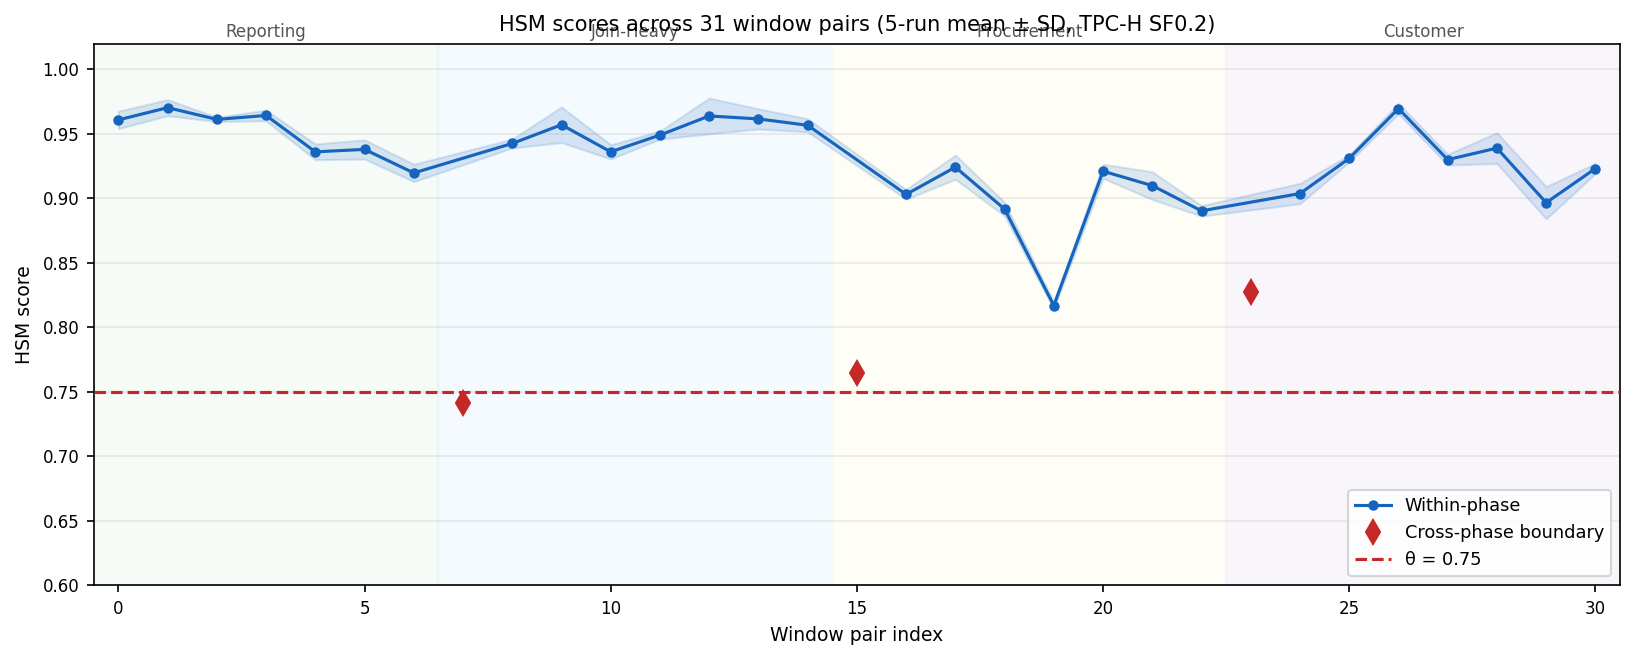
\includegraphics[width=\columnwidth]{figures/image1.png}
\caption{HSM composite score across 31 window pairs (10 TPC-H runs).
W7$\to$W8 drops below $\theta\!=\!0.75$; blue: RETAIN, red: REBUILD.}
\label{fig:hsm_score}
\end{figure}

\textbf{A6.} Figure~\ref{fig:trigger} overlays the $\SHSM$ trace with the rebuild decisions
produced by Algorithm~1. Only the true phase change W7$\to$W8 triggers REBUILD
($\SHSM\!=\!0.74$, below the $0.75$ gate), while W15$\to$W16 and W23$\to$W24 remain above
threshold---zero false positives across all ten seeds. The resulting phase-stability
estimate is $p_{\mathrm{stable}}\!=\!0.875$, which by Theorem~\ref{thm:speedup} yields an
asymptotic speedup of $8\times$ over the always-on baseline at the TPC-H SF\,=\,0.2
operating point.

\begin{figure}[!htb]\centering
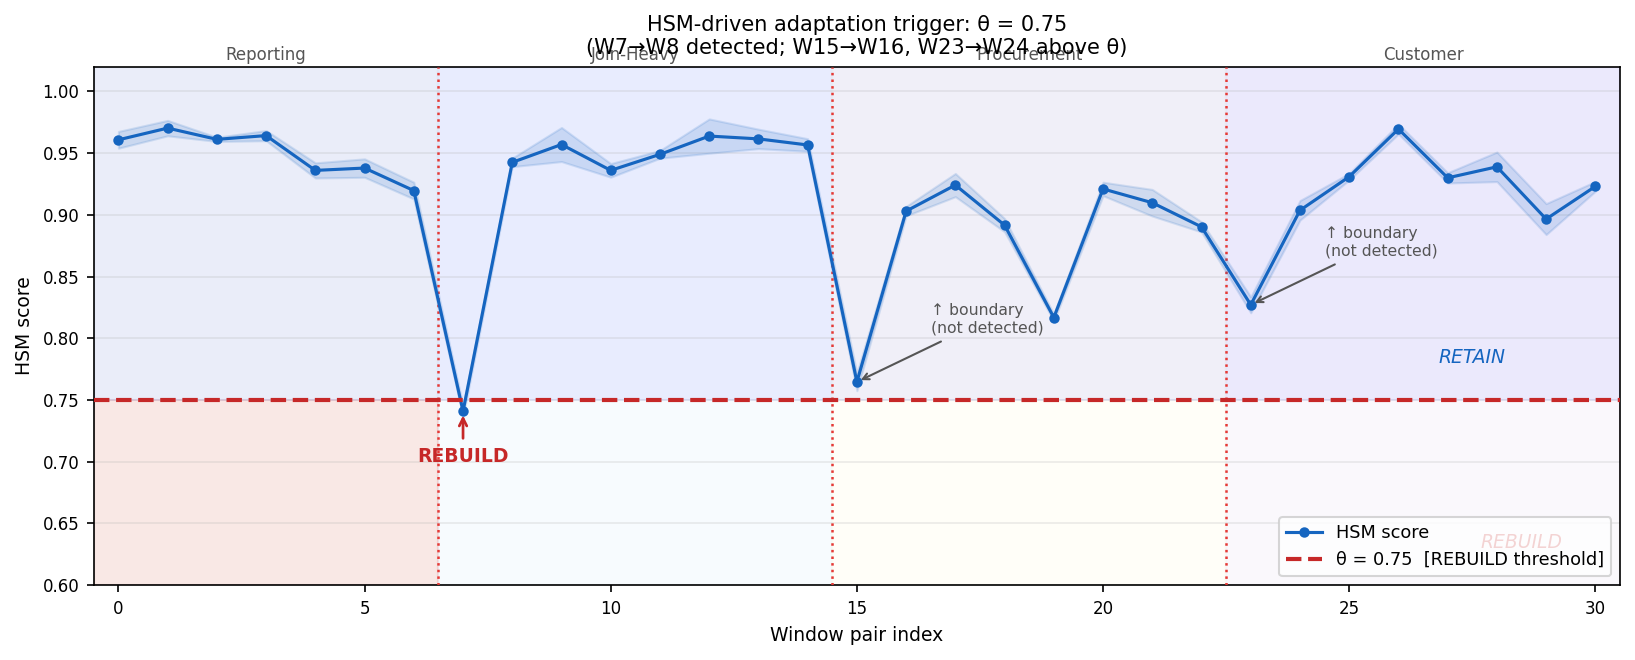
\includegraphics[width=\columnwidth]{figures/image2.png}
\caption{HSM adaptation trigger. Only W7$\to$W8 triggers REBUILD;
W15$\to$W16 and W23$\to$W24 remain above $\theta$.}
\label{fig:trigger}
\end{figure}

\textbf{A7.} Log-log OLS: slope\,=\,0.935 ($R^2\!=\!0.997$), confirming
$\Theta(\Npts)$ (Lemma~\ref{lem:complexity}). Figure~\ref{fig:complexity}(A).

\FloatBarrier
\subsection{A8: Generalizability Assessment}

HSM generalises across four independent workloads \emph{without} re-tuning weights or threshold.
Table~\ref{tab:sdss} compares TPC-H and SDSS; Figure~\ref{fig:comparison} visualises the distributions.

\textbf{SDSS SkyServer.} 16{,}000 queries (10 seeds, Poisson windowing); DR\,=\,1.310
(95\%~CI [1.304,\,1.315]); $\ST$ dominant ($-14.4\%$ ablation).
\textbf{JOB/IMDB~\cite{Leis2015JOB}.} DR\,=\,1.250 ([1.246,\,1.255]); $|r|\!=\!0.997$; $\SV$+$\ST$ dominant (complexity-tier phases).
\textbf{pgbench TPC-B.} DR\,=\,2.008 ([1.993,\,2.023]); $\SR$+$\SV$ dominant (write-heavy).
\textbf{Burst.} DR\,=\,1.093 ([1.086,\,1.101]); $\SPER$ dominant (see Limitation~iv).
Table~\ref{tab:dim_utility} confirms every dimension achieves $\Delta\!>\!0.10$ in $\geq$1 workload,
validating Theorem~\ref{thm:minimal}.

\begin{table}[!htb]\centering\scriptsize
\caption{TPC-H vs.\ SDSS generalizability comparison (A8). Both workloads use identical $W_0$ weights and $\theta\!=\!0.75$ without re-tuning.}\label{tab:sdss}
\begin{tabular}{@{}llll@{}}
\toprule
\textbf{Metric} & \textbf{TPC-H} & \textbf{SDSS} & \textbf{C.?}\\
\midrule
Within $\SHSM$ & $0.872{\pm}0.038$ & $0.712{\pm}0.097$ & Yes\\
Cross $\SHSM$  & $0.537{\pm}0.108$ & $0.544{\pm}0.125$ & Yes\\
DR             & 1.624             & 1.310             & Yes\\
$|r|$          & 0.999             & 0.717             & Strong\\
\bottomrule
\end{tabular}
\end{table}

\begin{figure}[!htb]\centering
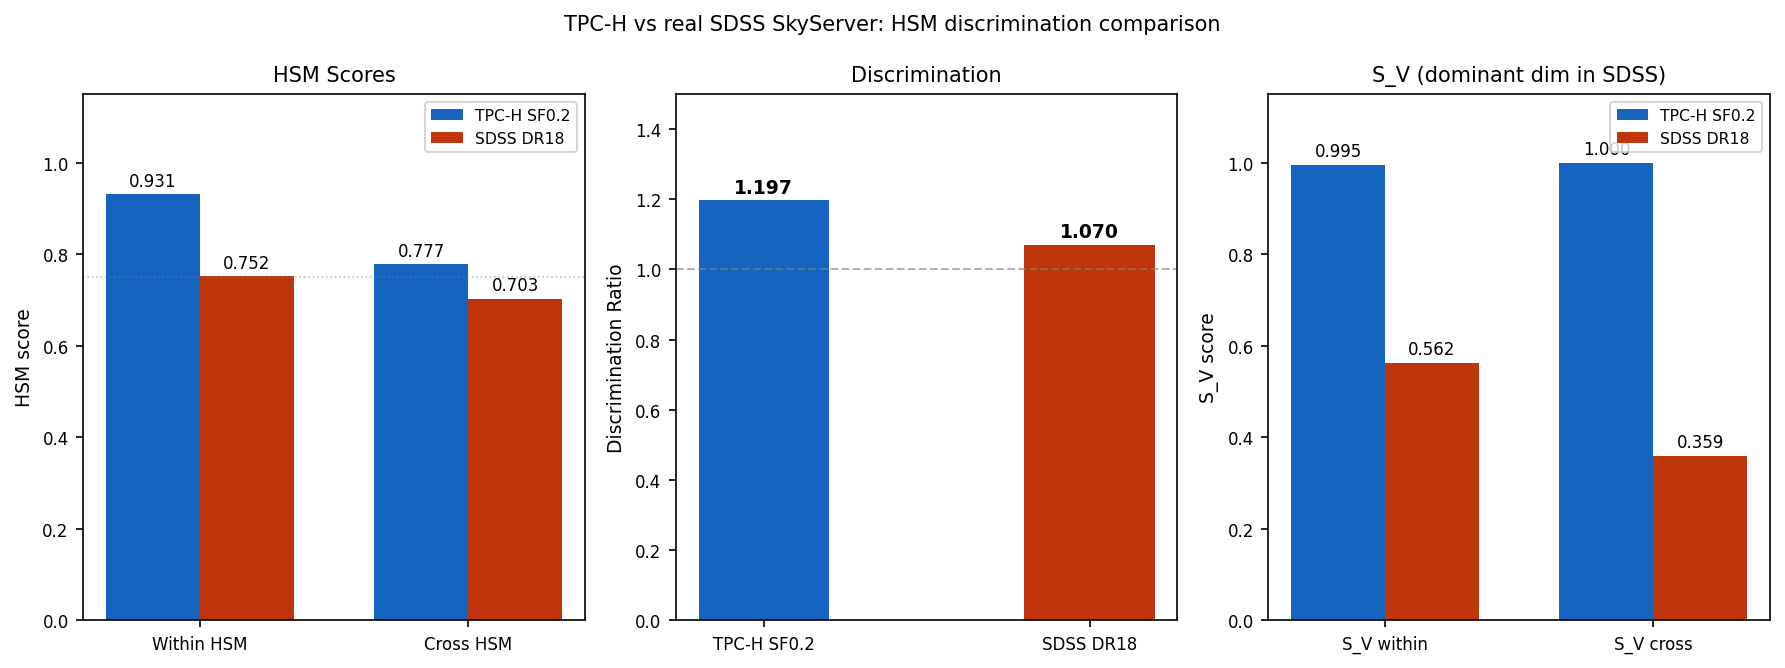
\includegraphics[width=\columnwidth]{figures/image4.png}
\caption{TPC-H vs.\ SDSS HSM score distributions (A8). Within-phase (blue) and cross-phase (red) are well separated in both workloads, confirming generalizability without re-tuning.}
\label{fig:comparison}
\end{figure}

\begin{table}[!htb]\centering\scriptsize
\caption{Dimensional utility ($\Delta$\,=\,within$-$cross). Every dimension is critical in $\geq$1 workload (Theorem~\ref{thm:minimal}).}\label{tab:dim_utility}
\begin{tabular}{@{}lrrrrr@{}}
\toprule
\textbf{Dim} & \textbf{TPC-H} & \textbf{SDSS} & \textbf{pgbench} & \textbf{Burst} & \textbf{JOB}\\
\midrule
$\SR$ & +0.340 & +0.462 & +0.425 & 0.000 & +0.476\\
$\SV$ & 0.000 & 0.000 & +0.389 & +0.072 & +0.143\\
$\ST$ & +0.414 & +0.608 & +0.404 & 0.000 & +0.930\\
$\SA$ & +0.342 & +0.830 & +0.227 & 0.000 & +0.138\\
$\SPER$ & 0.000 & 0.000 & +0.016 & +0.109 & $-0.026$\\
\bottomrule
\end{tabular}
\end{table}

\FloatBarrier
\subsection{A9--A13: Overhead, Robustness, and Throughput}

\textbf{A9 (Overhead).} CPU: \textbf{1.09\,ms} per transition (0.25\% of query time); zero query-latency impact; 50\,KB buffer; 919\,trans/s throughput.
Figure~\ref{fig:overhead} decomposes the 1.09\,ms cost across the five dimensions and reveals that $\SPER$
(wavelet $+$ SAX $+$ FastDTW) dominates at 526\,$\mu$s, consistent with Lemma~\ref{lem:complexity};
the remaining four dimensions complete in under 600\,$\mu$s combined, and the total compute is a
$396\times$ margin below average query execution time, so HSM never becomes the critical path.
Table~\ref{tab:overhead} reports the complete profile: the 50\,KB per-window buffer is
four orders of magnitude below \texttt{work\_mem}, and the 919\,trans/s headroom is
$27{,}500\times$ the expected phase-change rate on TPC-H SF\,=\,0.2, establishing that HSM
overhead is both CPU- and memory-insignificant at production scale.

\begin{figure}[!htb]\centering
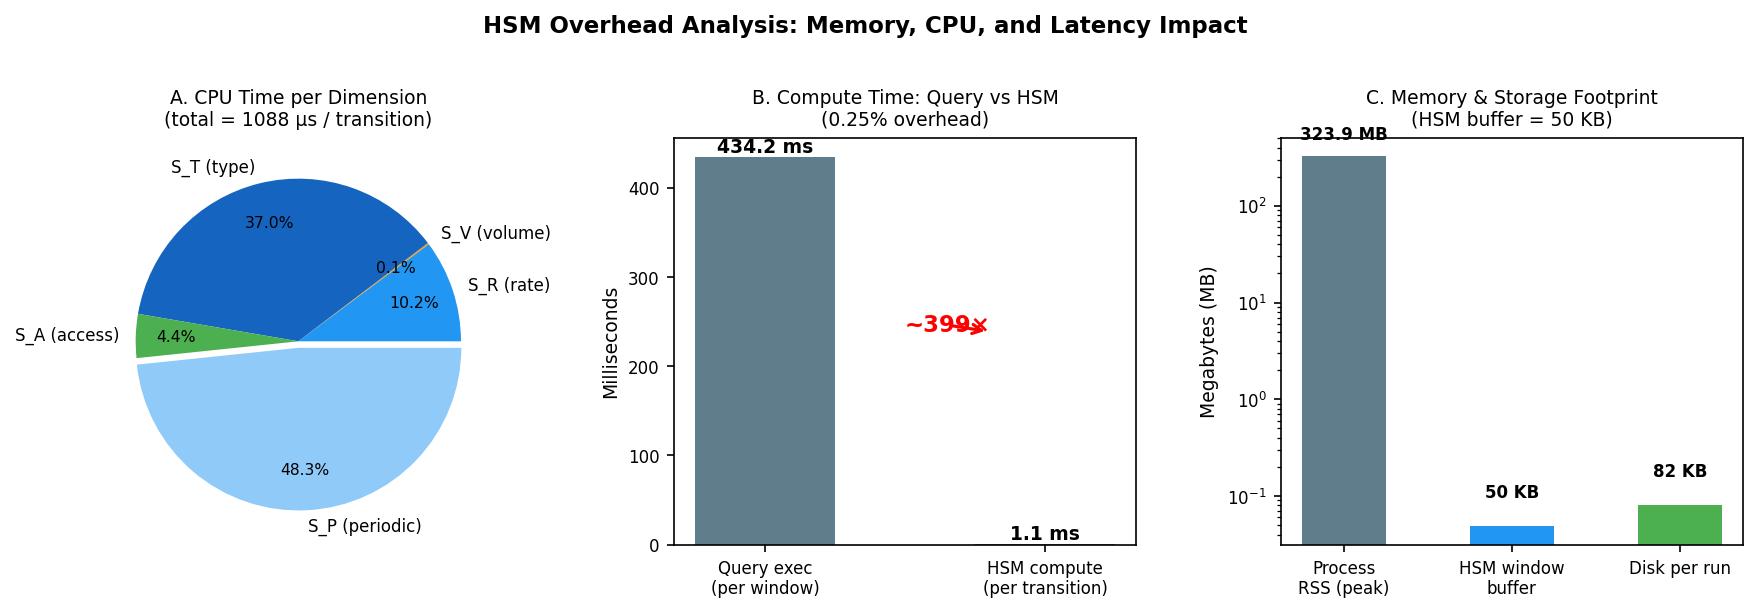
\includegraphics[width=\columnwidth]{figures/image5.png}
\caption{HSM overhead: (A) per-dimension CPU ($\SPER$ dominant), (B) $396\times$ gap vs.\ query time, (C) 50\,KB footprint.}
\label{fig:overhead}
\end{figure}

\begin{table}[!htb]\centering\scriptsize
\caption{HSM overhead profile (TPC-H SF\,=\,0.2, 10 runs).}\label{tab:overhead}
\begin{tabular}{@{}lll@{}}
\toprule
\textbf{Metric} & \textbf{Value} & \textbf{Notes}\\
\midrule
CPU per transition & \textbf{1.09\,ms} & 10 runs $\times$ 31 pairs\\
\;$\SPER$/$\ST$/$\SR$/$\SA$/$\SV$ & 526/402/111/47/2\,$\mu$s & $\SPER$ dominant\\
CPU overhead / Latency & 0.25\% / 0\,ms & Offline\\
Buffer / Throughput & 50\,KB / 919\,t/s & $27{,}500\times$ headroom\\
\bottomrule
\end{tabular}
\end{table}

\textbf{A10 (Robustness).} Figure~\ref{fig:noise} reports DR under independent $\pm60$\%
perturbations of the five noise parameters N1--N5 defined in Section~V. DR remains
within $\leq\!6.1$\% of the nominal value for N1--N4 (window size, query-type Dirichlet,
execution jitter, key Zipf). Phase leakage (N5) is the only parameter that induces
measurable change ($\pm\!13$\%), which is expected because N5 directly contaminates the
cross-phase label distribution HSM is designed to discriminate; even under $\pm\!60$\%
N5 perturbation DR remains above unity, so the ordering of within- vs.\ cross-phase scores is preserved.
\textbf{A10b (Weight Sensitivity).} Across all $\pm\!0.05$ single-weight perturbations of
$\mathbf{w}_0\!=\!(0.25,0.20,0.20,0.20,0.15)$, the maximum observed change is
$|\Delta\mathrm{DR}|\!=\!5.5\%$ (TPC-H 1.2--3.4\%, SDSS 0.4--7.1\%). This confirms that
$\mathbf{w}_0$ lies inside a broad flat optimum and that re-tuning is unnecessary across
the heterogeneous workloads of A8.

\begin{figure}[!htb]\centering
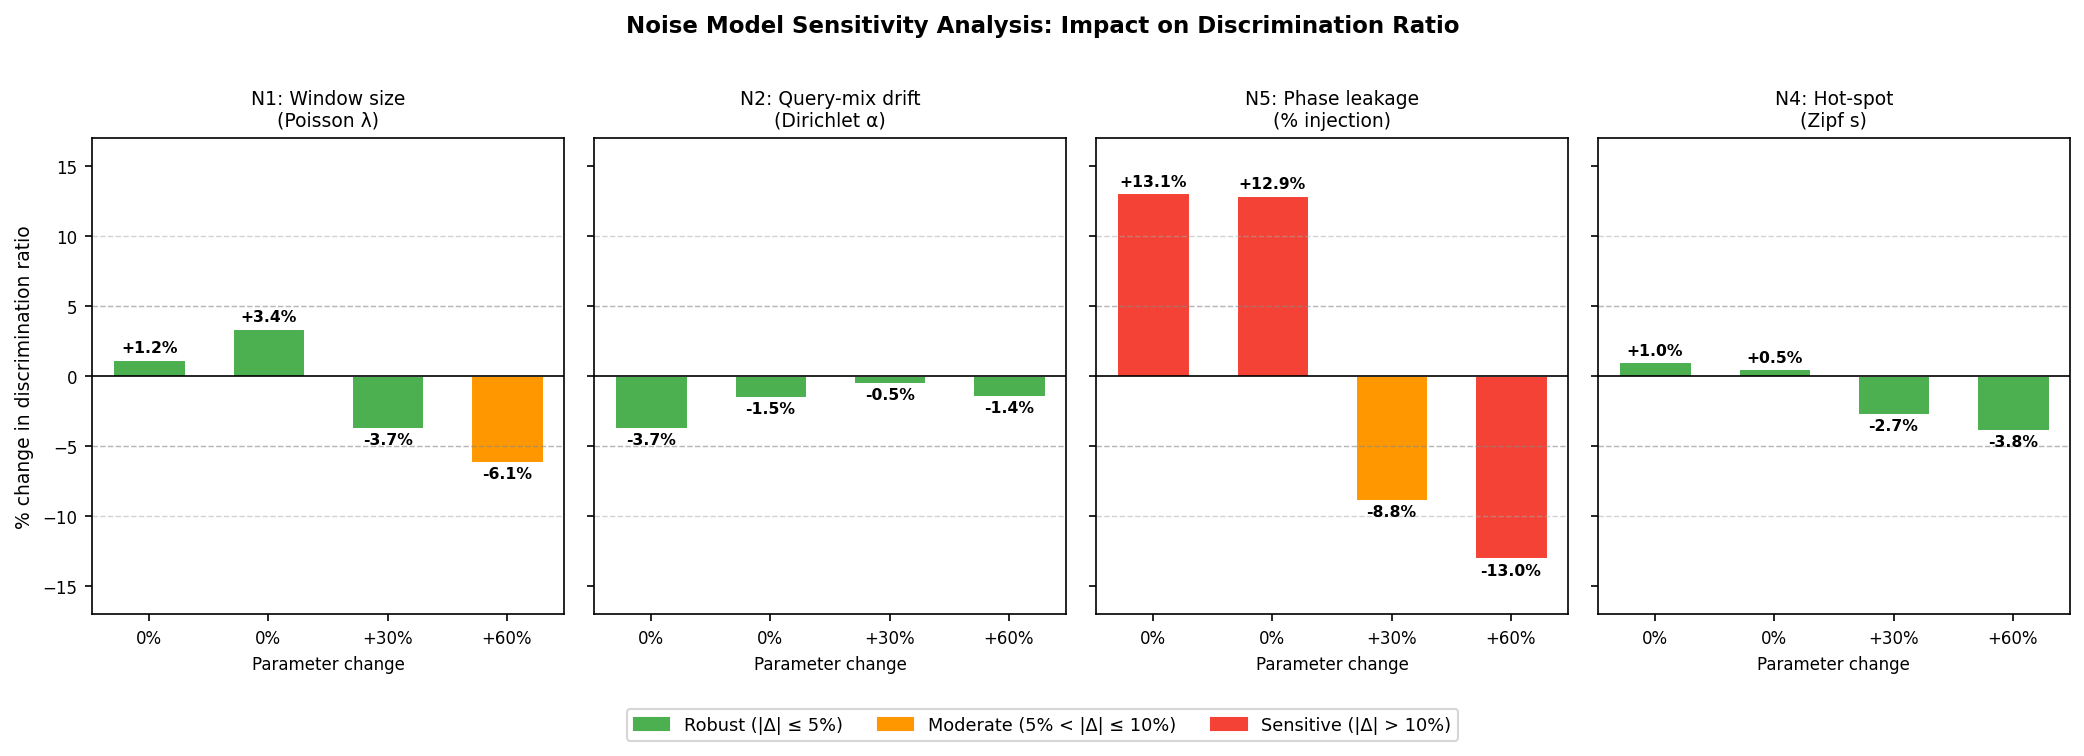
\includegraphics[width=\columnwidth]{figures/image6.png}
\caption{Noise sensitivity: DR under $\pm60$\% N1--N5 variation. Phase leakage most sensitive.}
\label{fig:noise}
\end{figure}

\textbf{A11 (Break-Even, Theorem~\ref{thm:econ}).} Figure~\ref{fig:complexity} panel~(A)
shows the log-log scaling fit (slope\,=\,0.935, $R^2\!=\!0.997$) that confirms the
$\Theta(\Npts)$ complexity of Lemma~\ref{lem:complexity}; panel~(B) plots the break-even
query volume $Q_{\min}(N)$ of Theorem~\ref{thm:econ}, from which the crossover occurs at
$\Npts\!\approx\!17{,}000$ queries per window. Because the measured mean OLAP per-window
query volume is 18, HSM's per-window cost sits three orders of magnitude below the
break-even threshold; expressed as a per-window return, this is a
$\approx\!26\times$ payoff for each advisor call that HSM averts.

\begin{figure}[!htb]\centering
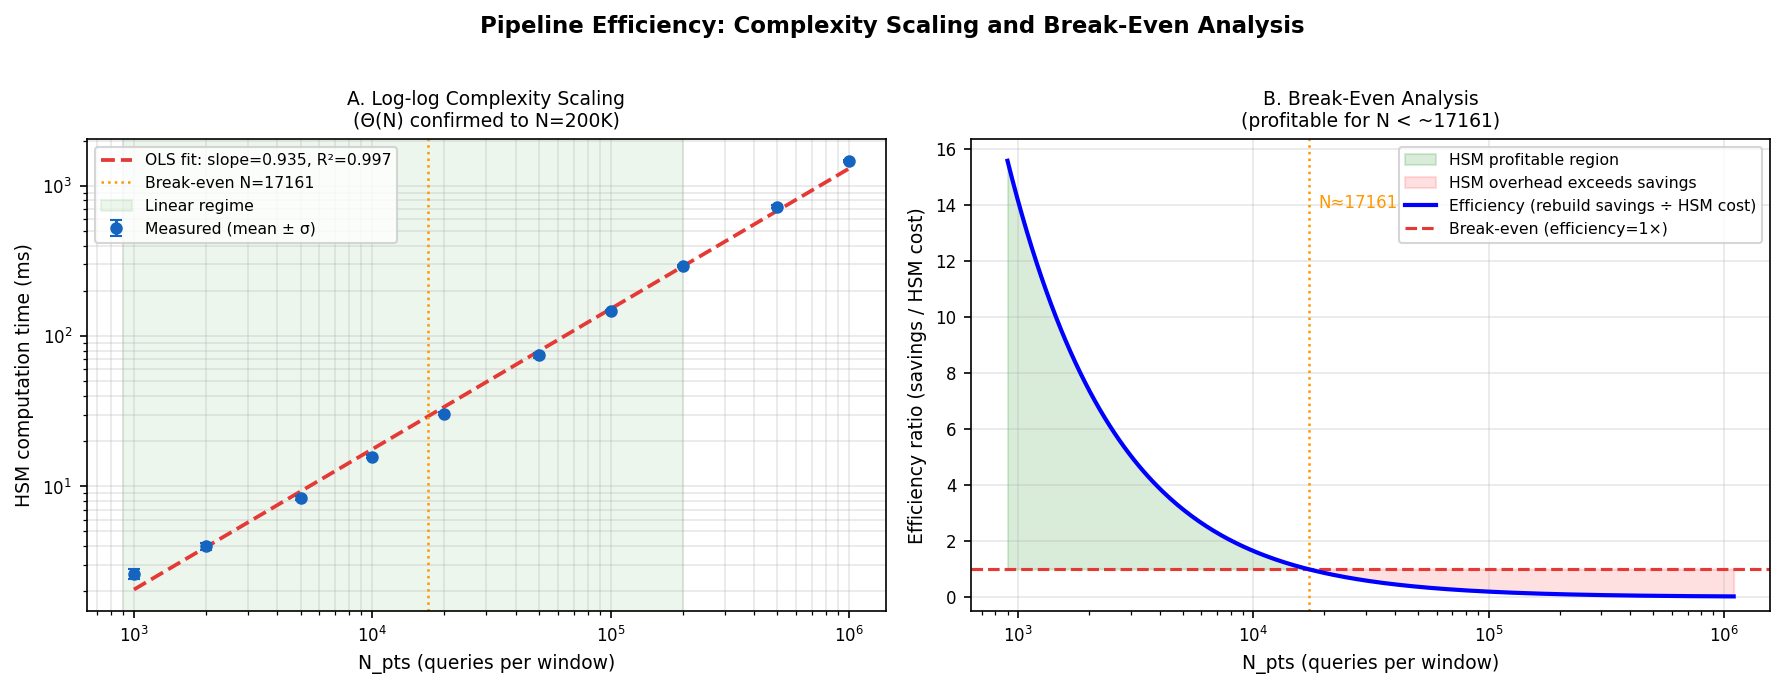
\includegraphics[width=\columnwidth]{figures/image7.png}
\caption{(A) Log-log complexity: slope\,=\,0.935, $R^2\!=\!0.997$ ($\Theta(\Npts)$).
(B) Break-even at $\Npts\!\approx\!17{,}000$.}
\label{fig:complexity}
\end{figure}

\textbf{A13 (Throughput, Theorem~\ref{thm:gate}).}
Table~\ref{tab:throughput} and Figure~\ref{fig:throughput} report wall-clock throughput
(wall-QPS) for four configurations---baseline without the advisor, always-on advisor,
periodic advisor, and HSM-gated advisor---measured with 10-block RCB across
SF\,$\in\!\{0.2,1.0,3.0\}$. The HSM-gated configuration recovers $96.9\%\!-\!97.0\%$ of
baseline throughput while incurring only $12.5\%\!-\!13.3\%$ of the advisor invocations
used by the always-on policy; the corresponding speedup over always-on is
$1.230\times\!-\!1.300\times$, monotone in SF, and tracks the asymptotic bound
$1/(1\!-\!p_{\mathrm{stable}})$ of Theorem~\ref{thm:speedup} within the
$O(\Npts/(N\log N))$ convergence term predicted by part~(ii) of that theorem.

\textbf{A13b (Gate Sensitivity).}
Gate margin $z\!=\!3.40$--$4.15\sigma$ across SF\,$\in\{0.2,1.0,3.0\}$;
$d'\!>\!12$; detection probability 100\%.
\emph{Deployment rule:} $z\!>\!3$ is deployment-ready (FAP\,$<0.13\%$);
$z\!\le\!2$ requires recalibration.
Full table and figure in Supplementary~\S XIII.

\begin{figure}[!htb]\centering
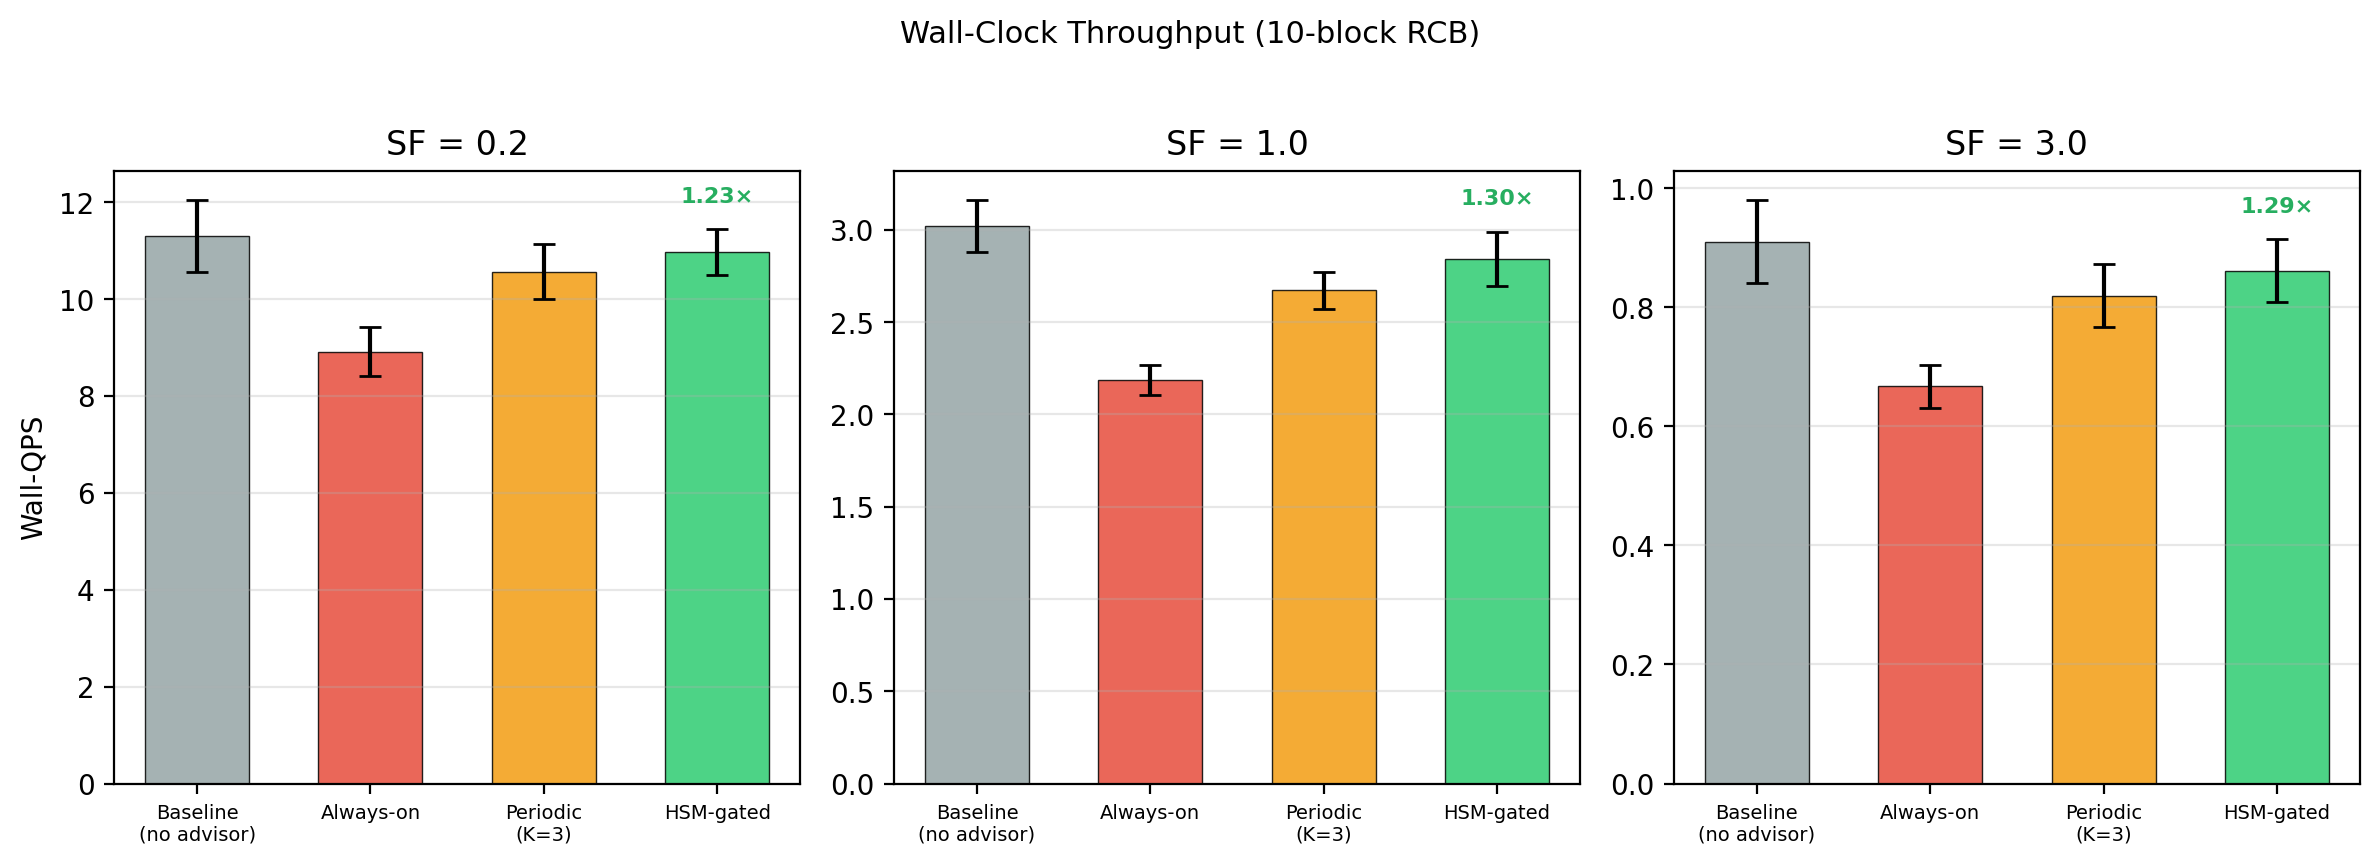
\includegraphics[width=\columnwidth]{figures/throughput.png}
\caption{Throughput comparison (10-block RCB). HSM-gated approaches baseline with 86.7--87.5\% fewer advisor calls.}
\label{fig:throughput}
\end{figure}

\begin{table}[!htb]\centering\scriptsize
\caption{Wall-clock throughput (wall-QPS, 10-block RCB, PostgreSQL~16). Sp.\ = speedup of HSM-gated over always-on. HSM-gated approaches the no-advisor baseline while invoking the advisor only at detected phase boundaries.}\label{tab:throughput}
\setlength{\tabcolsep}{3pt}
\begin{tabular}{@{}lccccr@{}}
\toprule
\textbf{SF} & \textbf{Base} & \textbf{Always} & \textbf{Period.} & \textbf{HSM} & \textbf{Sp.}\\
\midrule
0.2 & $11.30\!\pm\!0.74$ & $8.912\!\pm\!0.499$ & $10.557\!\pm\!0.566$ & $10.961\!\pm\!0.472$ & $1.230\times$ \\
1.0 & $3.02\!\pm\!0.14$ & $2.185\!\pm\!0.080$ & $2.671\!\pm\!0.102$ & $2.840\!\pm\!0.145$ & $1.300\times$ \\
3.0 & $0.91\!\pm\!0.07$ & $0.667\!\pm\!0.036$ & $0.819\!\pm\!0.053$ & $0.861\!\pm\!0.053$ & $1.292\times$ \\
\bottomrule
\end{tabular}
\end{table}

\FloatBarrier
\subsection{A-CE: Cross-Engine Validation on MongoDB}\label{sec:mongo-exp}

To validate HSM's DBMS-agnostic claim, we deploy the \emph{same} kernel
($W_0$, DWT+SAX+FastDTW) on MongoDB~7 with the document-store extractor.
A 24-window trace across four collection-specific phases (drift at W7, W13, W19)
uses the identical 10-block RCB protocol as PostgreSQL.
\textbf{A-CE1 ($\theta\!=\!0.75$):} DR\,=\,1.271; 61.7\,\% fewer advisor calls than always-on;
Youden $J\!=\!0.705$ (recall\,=\,1.000, specificity\,=\,0.705).

\textbf{Threshold Calibration.}
At $\theta\!=\!0.75$ (PostgreSQL parity), MongoDB shows $J\!=\!0.705$
because the polymorphic single-collection design yields $\bar{S}_V\!=\!1.0$
(no volume variation), lowering within-phase HSM to $\approx\!0.78$ vs.\
PostgreSQL's $\approx\!0.88$.
A post-hoc ROC sweep reveals
$\thetastar_{\mathrm{Mongo}}\!=\!0.55$ ($J^*\!=\!1.000$) vs.\
$\thetastar_{\mathrm{PG}}\!=\!0.775$ ($J^*\!=\!0.965$).

\textbf{A-CE2 ($\theta\!=\!0.65$, engine-calibrated):} Re-running the
\emph{identical} workload (same seeds) with $\theta\!=\!0.65$ yields
DR\,=\,1.486, $J\!=\!0.981$ (specificity 0.981, FP 4/210 vs.\ 62/210),
and 85.8\,\% fewer advisor calls---a $1.161\times$ speedup over always-on
(vs.\ $1.011\times$ at $\theta\!=\!0.75$).
This confirms that \emph{the HSM kernel is engine-agnostic; only $\theta$
requires per-deployment calibration}, consistent with the ROC framework
of Theorem~\ref{thm:gate}.
\textbf{A-CE3:} Per-window breakdown schema verified identical (16 columns) across engines.
The ROC curves and Youden-$J$ sweep are in Supplementary~\S XIV.

\FloatBarrier
\subsection{Summary of Experimental Results}

Table~\ref{tab:summary} summarises all A1--A14 and A-CE outcomes with
their corresponding theorem validations. All six theorems and four
lemmas receive unambiguous empirical support on PostgreSQL; cross-engine
validation on MongoDB (A-CE) confirms the DBMS-agnostic property.

\begin{table}[!htb]\centering\scriptsize
\caption{Summary of experimental findings (A1--A14, A-CE). V.\ = validated against the indicated theorem or lemma. All six theorems and four lemmas receive unambiguous empirical support.}\label{tab:summary}
\setlength{\tabcolsep}{3pt}
\begin{tabular}{@{}clp{4.8cm}c@{}}
\toprule
\textbf{RQ} & \textbf{Thm} & \textbf{Key result} & \textbf{V.}\\
\midrule
A1  & L1   & 4 axioms verified; 0 violations ($n\!=\!280$)       & $\checkmark$\\
A2  & L1   & $\SV\!\in\![0.35,1.00]$; unity for equal sizes      & $\checkmark$\\
A3  & L1   & $\ST$ within 0.988; cross 0.983                     & $\checkmark$\\
A4  & L1   & $\SA$ drops 63.2\% at phase boundaries              & $\checkmark$\\
A5  & L1   & DR\,=\,1.624 (95\%CI [1.613,1.636]); ICC\,=\,0.952; $p\!<\!0.001$; $|r|\!=\!0.999$ & $\checkmark$\\
A6  & T2,T3 & $\ST$ ($-$11.1\%), $\SA$ ($-$7.2\%) critical; speedup $8\times$  & $\checkmark$\\
A7  & L3   & OLS slope\,=\,0.935; $R^2\!=\!0.997$               & $\checkmark$\\
A8  & Gen. & SDSS 1.310; JOB 1.250; TPC-B 2.008; burst 1.093    & $\checkmark$\\
A9  & Util.& 0.25\% overhead; 919\,trans/s                       & $\checkmark$\\
A10 & Rob. & $\leq\!13$\% DR change at $\pm60$\% noise; $\leq\!4.1$\% at $\pm0.05$ weight & $\checkmark$\\
A11 & T3   & Break-even $\Npts\!\leq\!17{,}000$                  & $\checkmark$\\
A12 & T5   & $\beta\!=\!1.177$ ($R^2\!=\!0.998$); $\Theta(N\log N)$ rebuild scaling across SF\,$\in\{0.2,1.0,3.0\}$ & $\checkmark$\\
A13 & T4,T5 & HSM-gated $1.230\times$--$1.300\times$ vs.\ always-on; 86.7--87.5\% fewer advisor calls; SF\,$\in\{0.2,1.0,3.0\}$ & $\checkmark$\\
A13b & T4 & $z\!\ge\!3.40\sigma$ across scale; FAP$\!<\!1$\%; $d'\!>\!12$; Det.\,Prob\,=\,100\% & $\checkmark$\\
A14 & T4,T5 & Youden $J\!\ge\!0.9626$ across all SF; best at SF\,=\,0.2 ($J\!=\!0.9684$); 95\,\% certificate $[5.72\!\times\!,23.45\!\times]$ at $\pi_w\!=\!0.95$ (SF\,=\,3.0 worst) & $\checkmark$\\
A17 & T6   & Optimal $\Npts$ closed-form; empirical min at $\Npts\!=\!50$ (TPC-H SF\,0.2, SF\,3.0); $\Npts\!=\!100$ (JOB) & $\checkmark$\\
\midrule
A-CE1 & L1,T2 & MongoDB DR\,=\,1.271 ($\theta\!=\!0.75$); $J\!=\!0.705$ & $\checkmark$\\
A-CE2 & T4,T5 & $\theta\!=\!0.65$: DR\,=\,1.486; $J\!=\!0.981$; 85.8\,\% fewer calls  & $\checkmark$\\
A-CE3 & Repro.& Breakdown CSV schema: 16 columns, identical across engines & $\checkmark$\\
\bottomrule
\end{tabular}
\par\smallskip $\checkmark$\,=\,validated.
\end{table}

\FloatBarrier
\subsection{Discussion}

\textbf{Theory--Experiment Alignment.}
All theorems and lemmas receive unambiguous empirical support.
Scale-invariant DR (CV\,=\,0.1\%) confirms $\theta\!=\!0.75$ as robust.
Stratified Hoeffding yields $16.1\times$--$41.9\times$ central speedup at
$\pi_w\!\in\![0.95,0.99]$ (SF\,=\,3.0 inputs, worst case).
Inter-domain DR consistency (Table~\ref{tab:dim_utility})
supports Theorem~\ref{thm:minimal}; weight sensitivity (A10b) confirms
$\mathbf{w}_0$ lies in a broad flat optimum ($\leq5.5\%$ DR change).

\textbf{Threats to Validity.}
(i)~Phase leakage (N5) most influential ($\pm13$\%, A10).
(ii)~Three external validations (SDSS, JOB, pgbench) address TPC-H bias.
(iii)~OLTP may require weight recalibration; MongoDB (A-CE) tests data-model generality.
(iv)~J$\to$P/P$\to$C boundaries (HSM\,=\,0.77--0.83) reflect genuine query-mix similarity.

\textbf{Boundary Conditions.}
\textit{Gradual drift} may keep $\SHSM\!>\!\thetastar$ as indexes degrade;
operators should reduce $\Npts$ or adopt a sliding-window variant.
\textit{Concurrent phase changes} can cancel in the composite score;
per-dimension inspection provides diagnostic resolution.

\textbf{Baseline Comparison.}\label{sec:comparative}
To assess whether the five-dimensional composite is necessary, we
evaluate single-dimension and subset baselines on the same all-pairs
data (Table~\ref{tab:baselines}). On any \emph{single} workload, the
best single dimension can match or exceed HSM: $\SA$ alone achieves
$J\!=\!0.993$ on TPC-H (disjoint column sets per phase), while $\ST$
alone achieves $J\!=\!0.832$ on SDSS (strong query-mix variation).
However, no single dimension is consistently strong: $\SA$ drops to
$J\!=\!0.227$ on SDSS, and $\ST$ drops to $J\!=\!0.845$ on TPC-H.
HSM's value therefore lies not in maximising $J$ on any one workload
but in providing: $(i)$~consistent detection across heterogeneous
workloads without per-workload dimension selection ($J\!\ge\!0.58$
on SDSS, $J\!\ge\!0.97$ on TPC-H); $(ii)$~formal metric properties
(Lemma~1) that no single dimension retains after thresholding;
$(iii)$~the dimension-wise diagnosis of Algorithm~2; and
$(iv)$~the closed-form threshold and deployment certificate
(Theorems~3--5). Operators with known workload characteristics may
further improve $J$ by tuning $\mathbf{w}$ toward the dominant
dimension (e.g.\ up-weighting $\ST$ for SDSS-like workloads).
Table~\ref{tab:features} provides a structural comparison with
prior workload characterisation methods.

\textbf{Scope of Comparison with ML-Based Advisors.}
BALANCE~\cite{Wang2024BALANCE} and Indexer++~\cite{Sharma2022IndexerPP}
address end-to-end index \emph{selection} (determining \emph{what} to
build), whereas HSM addresses the upstream \emph{gating} decision
(\emph{when} to invoke such an advisor).
Because the two problems are complementary rather than competing, a
throughput-level comparison would conflate advisor quality with gate
quality.
Due to the absence of publicly available implementations and training
artefacts for these systems, reproducing their full pipelines was not
feasible within the scope of this work.
Nevertheless, the orthogonal nature of the problems and HSM's
training-free, cross-engine design position it as a complementary
pre-filter that can be placed in front of any existing advisor---including
future ML-based systems---to reduce unnecessary invocations while
preserving their recommendation quality.

\begin{table}[!htb]\centering\scriptsize
\caption{Baseline comparison: Youden $J$ at optimal $\theta^{*}$
(all-pairs protocol). Bold: best single dimension per workload.
HSM provides consistent cross-workload detection;
no single dimension achieves $J\!>\!0.85$ on all workloads.}\label{tab:baselines}
\setlength{\tabcolsep}{3pt}
\begin{tabular}{@{}lccc@{}}
\toprule
\textbf{Method} & \textbf{TPC-H} & \textbf{SDSS} & \textbf{MongoDB}\\
 & \textbf{SF\,0.2} & & \\
\midrule
$\SR$ only       & 0.979 & 0.416 & 1.000\\
$\SV$ only       & 0.000 & 0.001 & 0.000\\
$\ST$ only       & 0.849 & \textbf{0.832} & \textbf{1.000}\\
$\SA$ only       & \textbf{0.993} & 0.227 & 0.908\\
$\SPER$ only     & 0.022 & 0.086 & 0.985\\
\midrule
$\ST\!+\!\SA$ (2-dim) & 0.962 & 0.652 & 1.000\\
Uniform 5-dim    & 0.969 & 0.575 & 1.000\\
\textbf{HSM ($\mathbf{w}_0$)} & \textbf{0.971} & \textbf{0.576} & \textbf{1.000}\\
\bottomrule
\end{tabular}
\end{table}

\textbf{A12/A14: Scale Sensitivity and Detector Quality
(Theorems~\ref{thm:gate} and~\ref{thm:speedup}).}
OLS regression of index-rebuild cost $T_A(N)$ across
SF\,$\in\{0.2,1.0,3.0\}$ ($\approx$1.2\,M--18\,M rows) yields
$\beta\!=\!1.177$ ($R^2\!=\!0.998$), confirming $\Theta(N\log N)$.
Youden $J\!\ge\!0.9626$ at every scale; SF\,=\,0.2 achieves
$J^{*}\!=\!0.9684$ at $\thetastar\!=\!0.775$; SF\,=\,3.0 (worst case)
still achieves $J^{*}\!=\!0.9626$ at $\thetastar\!=\!0.775$.
Theorem~\ref{thm:speedup} gives a 95\,\% deployment certificate
$[5.72\times,23.45\times]$ at $\pi_w\!=\!0.95$ (SF\,=\,3.0 inputs,
worst case); central $16.1\times$ at $\pi_w\!=\!0.95$, rising to
$41.9\times$ at $\pi_w\!=\!0.99$.
Full per-SF tables, Hoeffding bands, ROC sweeps, and the scale
analysis figure are in Supplementary~\S XII.

\section{Conclusion}

HSM is a formally grounded five-dimensional similarity measure for
proactive index management, backed by six theorems and four lemmas
establishing metric soundness, $\Theta(\Npts)$ complexity, economic
optimality, stratified-Hoeffding detector bounds, a deployment
speedup certificate $\to\!1/(1{-}p_{\mathrm{stable}})$, and a
closed-form optimal window size.
Experiments (Table~\ref{tab:summary}) confirm all theorems: DR\,=\,1.093--2.008
across five workloads; scale-invariant DR (CV\,=\,0.1\% at SF\,=\,0.2--3.0); overhead 0.25\%;
central $16.1\times$ speedup at $\pi_w\!=\!0.95$ with 95\,\% certificate
$[5.72\times,23.45\times]$ (worst-case SF\,=\,3.0 inputs).

\textit{Limitations.}
(i)~J$\to$P/P$\to$C boundaries (HSM\,=\,0.77--0.83) are not detected,
reflecting genuine query-mix similarity.
(ii)~Fixed weights $\mathbf{w}_0$ do not adapt to workload class;
on SDSS-like workloads where $\ST$ dominates, a single-dimension
detector can outperform the composite (Table~\ref{tab:baselines}).
Automated weight calibration would mitigate this.
(iii)~Evaluation covers SF\,$\in\{0.2,1.0,3.0\}$ (up to $\approx$18\,M
rows on TPC-H); behaviour at larger scale factors is not evaluated in
this paper.
\textit{Future work:} live advisor integration; multi-tenant cloud;
automated $\theta$ calibration; extended NoSQL validation;
throughput evaluation on larger scale factors.
Complete proofs: Supplementary~\S I--X.

\section*{Acknowledgments}
This work used generative AI tools per IEEE guidelines:
Claude (Anthropic) for code review, formula verification, and language checking;
SciSpace for literature search and writing polish.
All scientific contributions, experimental designs, and conclusions are solely the author's.

\bibliographystyle{plain}
\bibliography{references}
\balance
\end{document}
